\chapter{High Multiplicity Jets at \texttt{ATLAS}}
\label{chap:ATLAS}

	Here we present the results of a complex experimental study of the effects of jet vetoes and
	azimuthal decorrelations in dijet events~\cite{Aad:2014pua}.  High Energy Jets is compared
	to both data and state-of-the-art fixed-order perturbative QCD predictions (supplemented with
	radiation by merging with a parton shower) from \texttt{POWHEG+
	PYTHIA8} and \texttt{POWHEG+HERWIG} (both implemented through the \texttt{POWHEG BOX} package
	\cite{1126-6708-2004-11-040}).

	The data compared to are 7~TeV proton-proton collisions as observed by the ATLAS
	experiment in two distinct data sets referred to as 2010 data and 2011 data.  The
	experimental cuts applied to these data sets differs and both are outlined in table
	\eqref{tab:atlasPcuts}.

	\begin{table}[bth]
	  \centering
	  \begin{tabular}{|l|c|}
	    \hline
	    2010 Jets (anti-$k_T$, 0.6) & $p_{Tj}>20$~GeV, \; $|y_j|<4.4$ \\
	    & $p_{T1}> 60.0$~GeV, \; $p_{T2}> 50.0$~GeV, \; \\
	    & $Q_0=20$~GeV \\
	    \hline
	    2011 Jets (anti-$k_T$, 0.6) & $p_{Tj}>30$~GeV, \; $|y_j|<2.4$ \\
	    & $p_{T1}> 60.0$~GeV, \; $p_{T2}> 50.0$~GeV \\
	    & \; $Q_0=30$~GeV, \; $\Delta y_{jj}>1.0$\\
	\hline
	  \end{tabular}
	  \caption{Cuts applied to theory simulations in the ATLAS dijets analyses.
	  $Q_0$ is the gap jet veto scale. The results are shown in
	  figs.~\eqref{fig:atlasPJ1}--\eqref{fig:atlasPJ6}.}
	  \label{tab:atlasPcuts}
	\end{table}

	This study focused on additional jet activity in dijet where the dijet system
	is constructed using the two leading jets in $p_T$.  These two jets are required
	to be significantly harder than any additional jets with extra cuts on the leading
	and sub-leading jets of $50$~GeV and $60$~GeV respectively.  After tagging the two
	leading jets in the event and considering all other jet radiation in the rapidity
	interval bounded by the dijets as a QCD correction.  Within in the two data sets
	defined in table \eqref{tab:atlasPcuts} a further subdivision was made.  For both the
	2010 and 2011 data a subset of events was defined by vetoing events with extra
	QCD radiation in the rapidity interval bounded by the dijet system above some veto
	scale $Q_0$.  It should also be noted that the 2011 data set required a minimum
	rapidity gap of 1.0 between all jets (for both cases with and without the gap jet
	veto) in order to encourage a rapidity span in to which extra radiation may arise.
	The full breakdown of this analysis then is in to four event categories;
	2010 data with and without a veto applied to gap jets and the 2011 data with and
	without a veto applied to gap jets.

	The predictions for these analyses generated by the High Energy Jets collaboration
	are given for both the partonic \HEJ calculation (shown in green in this chapter)
	and the \HEJA calculation (shown in orange).
	\ARIADNE is a parton shower package based on the Lund colour cascade dipole model.
	Due to the steps in this interfaced package necessary to remove the double counting
	(which arises from \HEJ and \ARIADNE both generating soft radiation) generating large
	data samples which can be used to give statistically significant predictions is
	\emph{extremely} computationally demanding.  In a standard partonic \HEJ run we
	evaluate the matrix element for each event at 76 different scale choices (since
	we allow for four choices of `central' scale and 19 combinations of the renormalisation
	scale, $\mu_r$, and factorisation scale, $\mu_f$ based on each central choice).
	After we chose a central scale (this choice is done while blind to the data for
	fairness) one set of these 19 scales combinations form an `envelope' of predictions
	for each bin in each plot - this spread is then represented by the green bands shown
	in the figs.~\eqref{fig:atlasPJ1}--\eqref{fig:atlasPJ6}.
	However, because of the structure of the matrix element evaluations within \HEJA
	we can only afford one scale choice per event and, as such, we cannot provide
	scale variation uncertainty bands with our showered numbers.  To be clear this
	is not a limitation of the physics since it is entirely possible to evaluate
	each matrix element multiple times - it is a computational consideration. \footnote{
	As seen in chapter \eqref{chap:Zs}, the renormalisation scale appears in a non-trivial way
	in the High Energy Jets matrix element.  It is contained implicitly in the strong coupling
	constant which is contained within the virtual corrections exponential.  As such
	we cannot simply generate predictions at a single scale and then reweight events
	at the post-analysis level.  In principle, we \emph{could} do this for our PDF
	evaluations though in practise this is very computationally cheap and therefore we
	chose not to.}  The orange bands shown with the \HEJA predictions throughout this
	chapter are the statistical bands (shown, as usual, at the 68\% confidence level).

	Observables were studied
	as a function of two properties of the dijets.  The rapidity gap between the dijets,
	$\Delta y$, and the mean traverse momenta of the dijet system, $\overline{p_T}$.\\
	Na\"ively for small $\Delta y$ we expect to see very little gap jets since there is
	a limited region in which extra jets may be clustered before they are clustered in
	to the dijet system itself.   Conversely, as we pull the dijets apart in rapidity
	we expect to see an increase in additional QCD radiation (since there is a larger
	phase space in which to radiate).  Similarly for $\overline{p_T}$, we expect that
	events with harder dijet systems will have higher gap activity simply because they
	have more energy available to radiate away in to additional jets.

	Throughout the remainder of this chapter the (a) sub-figures show data and
	predictions for the 2010 data set with respect to the rapidity span of the dijet
	system, $\Delta y$, while the (b) sub-figures show data and
	predictions from the 2011 data set with respect to the mean transverse momenta
	of the dijet system, $\overline{p_T}$.

	We begin by discussing the gap fraction, $f(Q_0)$, defined as:

	\begin{equation}
		f(Q_0) = \frac{\sigma_{jj}(Q_0)}{\sigma_{jj}},
	\end{equation}

	where $\sigma_{jj}(Q)$ is the total dijet cross section and $\sigma_{jj}(Q_0)$ is the dijet
	cross section passing the veto on additional gap scales for a scale choice $Q_0$.  Fig.
	\eqref{fig:atlasPJ1} shows the gap fraction with a veto scale of $20$~GeV in
	fig.~\eqref{fig:atlasPJ1a} and a veto scale of $30$~GeV in fig.~\eqref{fig:atlasPJ1b}.
	The behaviour observed is in line with our na\"ive guess discussed previously since the
	gap fraction decreases at both large $\Delta y$ and large $\overline{p_T}$.  We can see the
	best description of both data sets is given by \HEJA (excluding two very high $\overline{p_T}$
	bins where the predictions from \HEJA are visibly statistically limited). The partonic \HEJ
	prediction overshoots both data sets meaning that we underestimate the jet activity in the
	gap region while the predictions from \texttt{POWHEG} plus parton showers overestimate the
	QCD radiation here.  From fig. \eqref{fig:atlasPJ1} it is clear that in this situation it
	is not sufficient to only describe the wide-angle logarithmically enhanced terms resummed
	within the High Energy Jets framework and that the soft and collinear logarithms added by
	interfacing to \ARIADNE play a very important r\^ole.  It is visible from fig.~\eqref{fig:atlasPJ1}
	that the scale variations shown in \emph{partonic} \HEJ (since the \HEJA bands are statistical
	only) are quite significantly bigger than that shown by the other predictions.  This is
	expected since we only include matching up to leading-order whereas \texttt{POWHEG} is
	formally NLO accurate; it is well observed that as we include higher order terms (in the
	fixed order sense) we gain a better control of the scale uncertainties.

	\begin{figure}[bth]
		\centering
		\begin{subfigure}[b]{0.48\textwidth}
			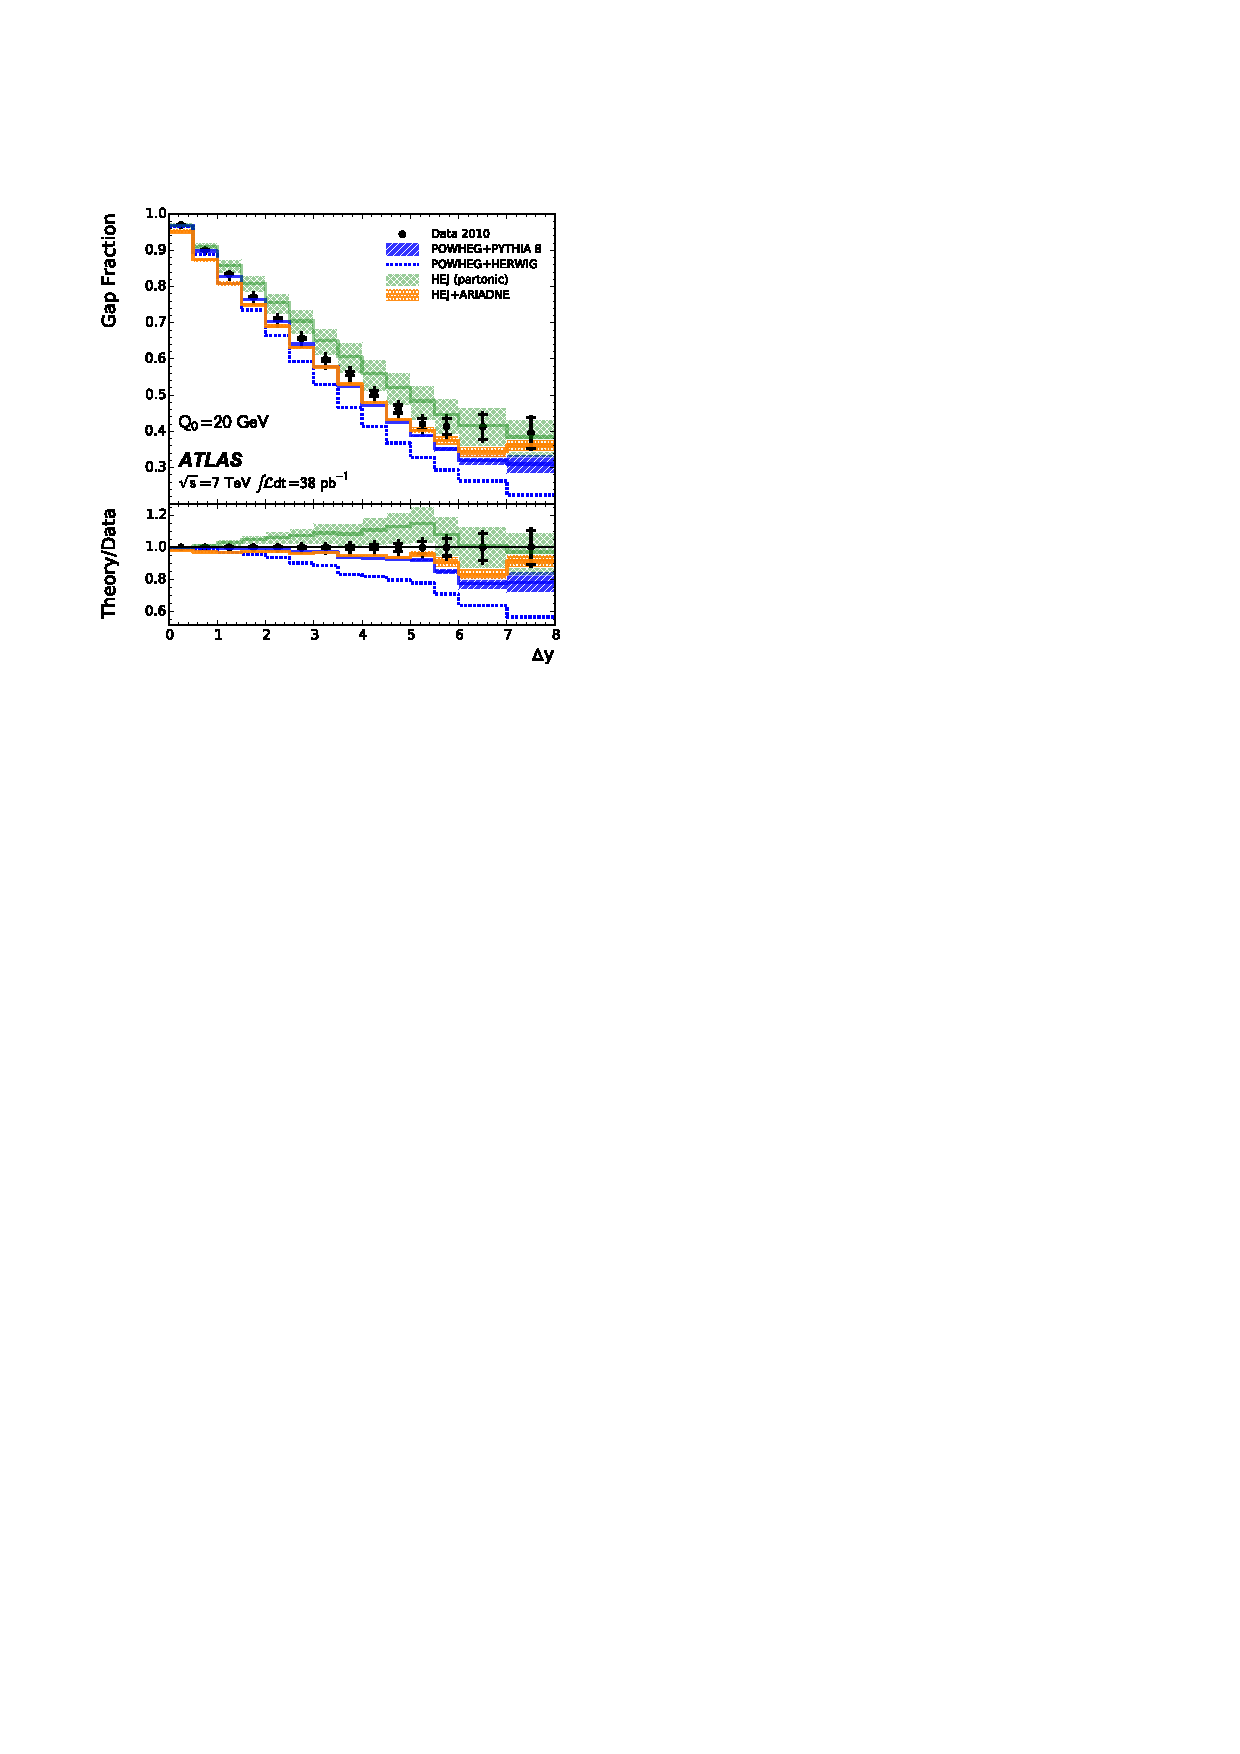
\includegraphics[width=\textwidth, height=1.0\textwidth]{pureJets3a}
			\caption{}
			\label{fig:atlasPJ1a}
		\end{subfigure}
		~
		\begin{subfigure}[b]{0.48\textwidth}
			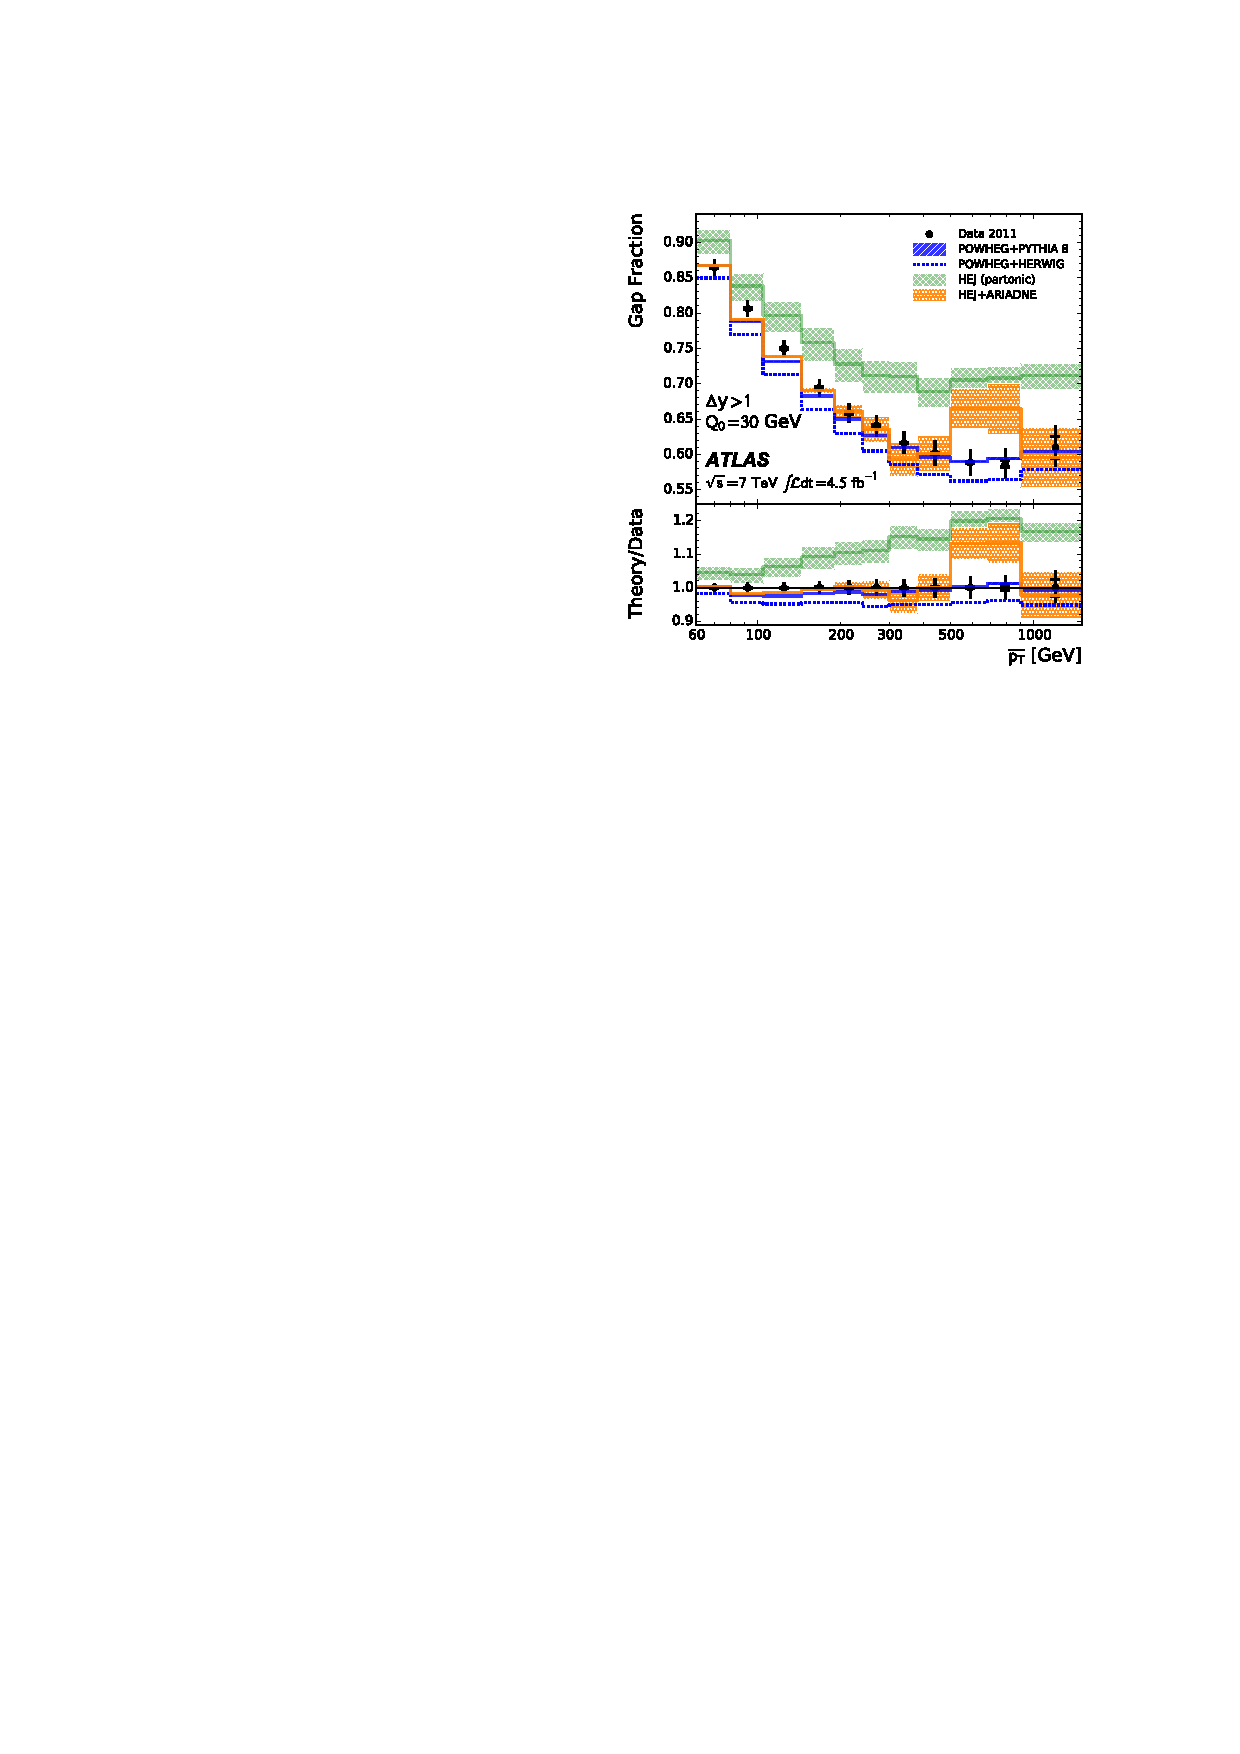
\includegraphics[width=\textwidth, height=1.0\textwidth]{pureJets3b}
			\caption{}
			\label{fig:atlasPJ1b}
		\end{subfigure}
		\caption{The gap fraction, $f(Q_0)$, as a function of (a) the rapidity gap,
		$\Delta y$, and (b) the average $p_T$, $\overline{p_T}$, of the dijet system.}
		\label{fig:atlasPJ1}
	\end{figure}

	Similarly, when we study the mean number of jets in the rapidity interval shown for in
	fig.~\eqref{fig:atlasPJ2} we see that \HEJA and \texttt{POWHEG+PYTHIA8} give the best
	description of the data.  Once again the partonic \HEJ prediction undershoots the data
	significantly when describing both of the dijet characteristics while \texttt{POWHEG+HERWIG}
	overestimates the jet activity.

	\begin{figure}[bth]
		\begin{subfigure}[b]{0.48\textwidth}
			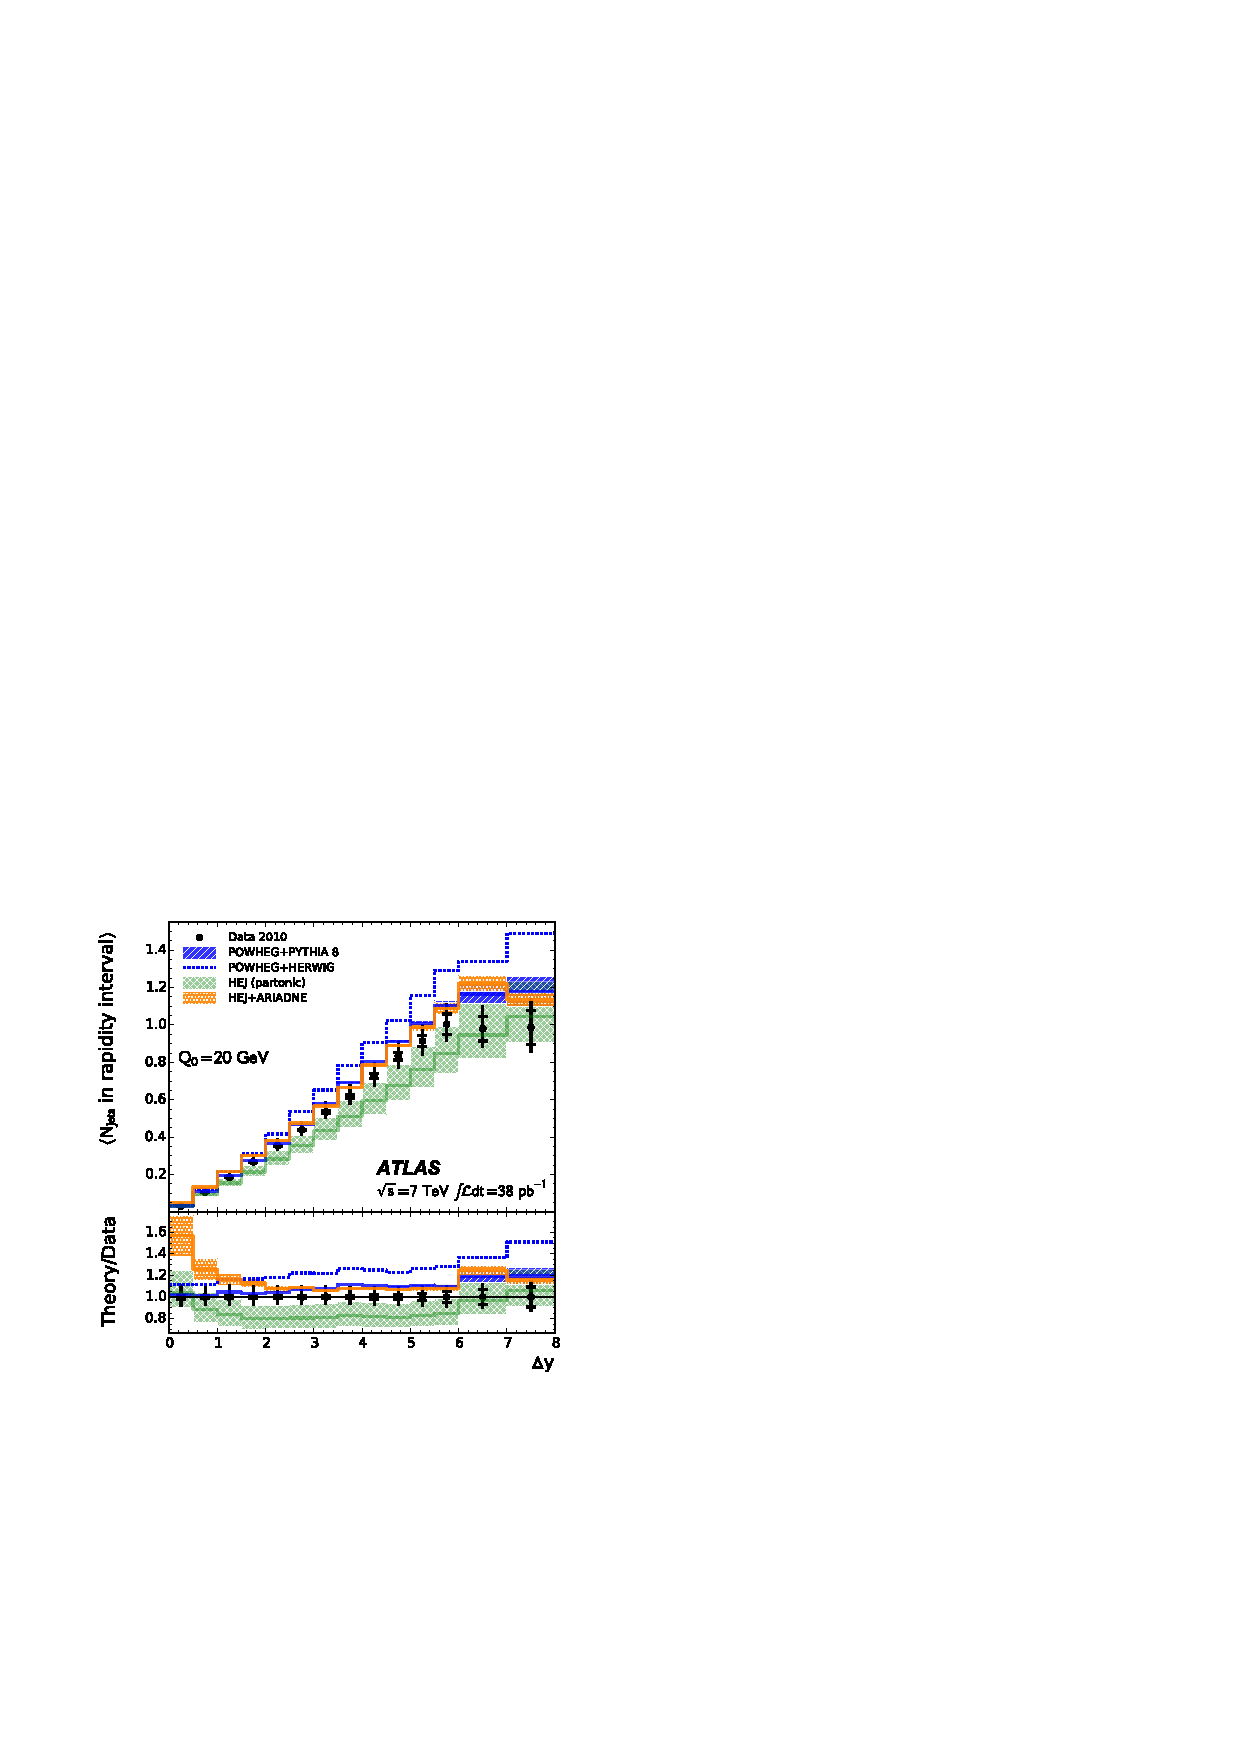
\includegraphics[width=\textwidth, height=1.0\textwidth]{pureJets4a}
			\caption{}
			\label{fig:}
		\end{subfigure}
		~
		\begin{subfigure}[b]{0.48\textwidth}
			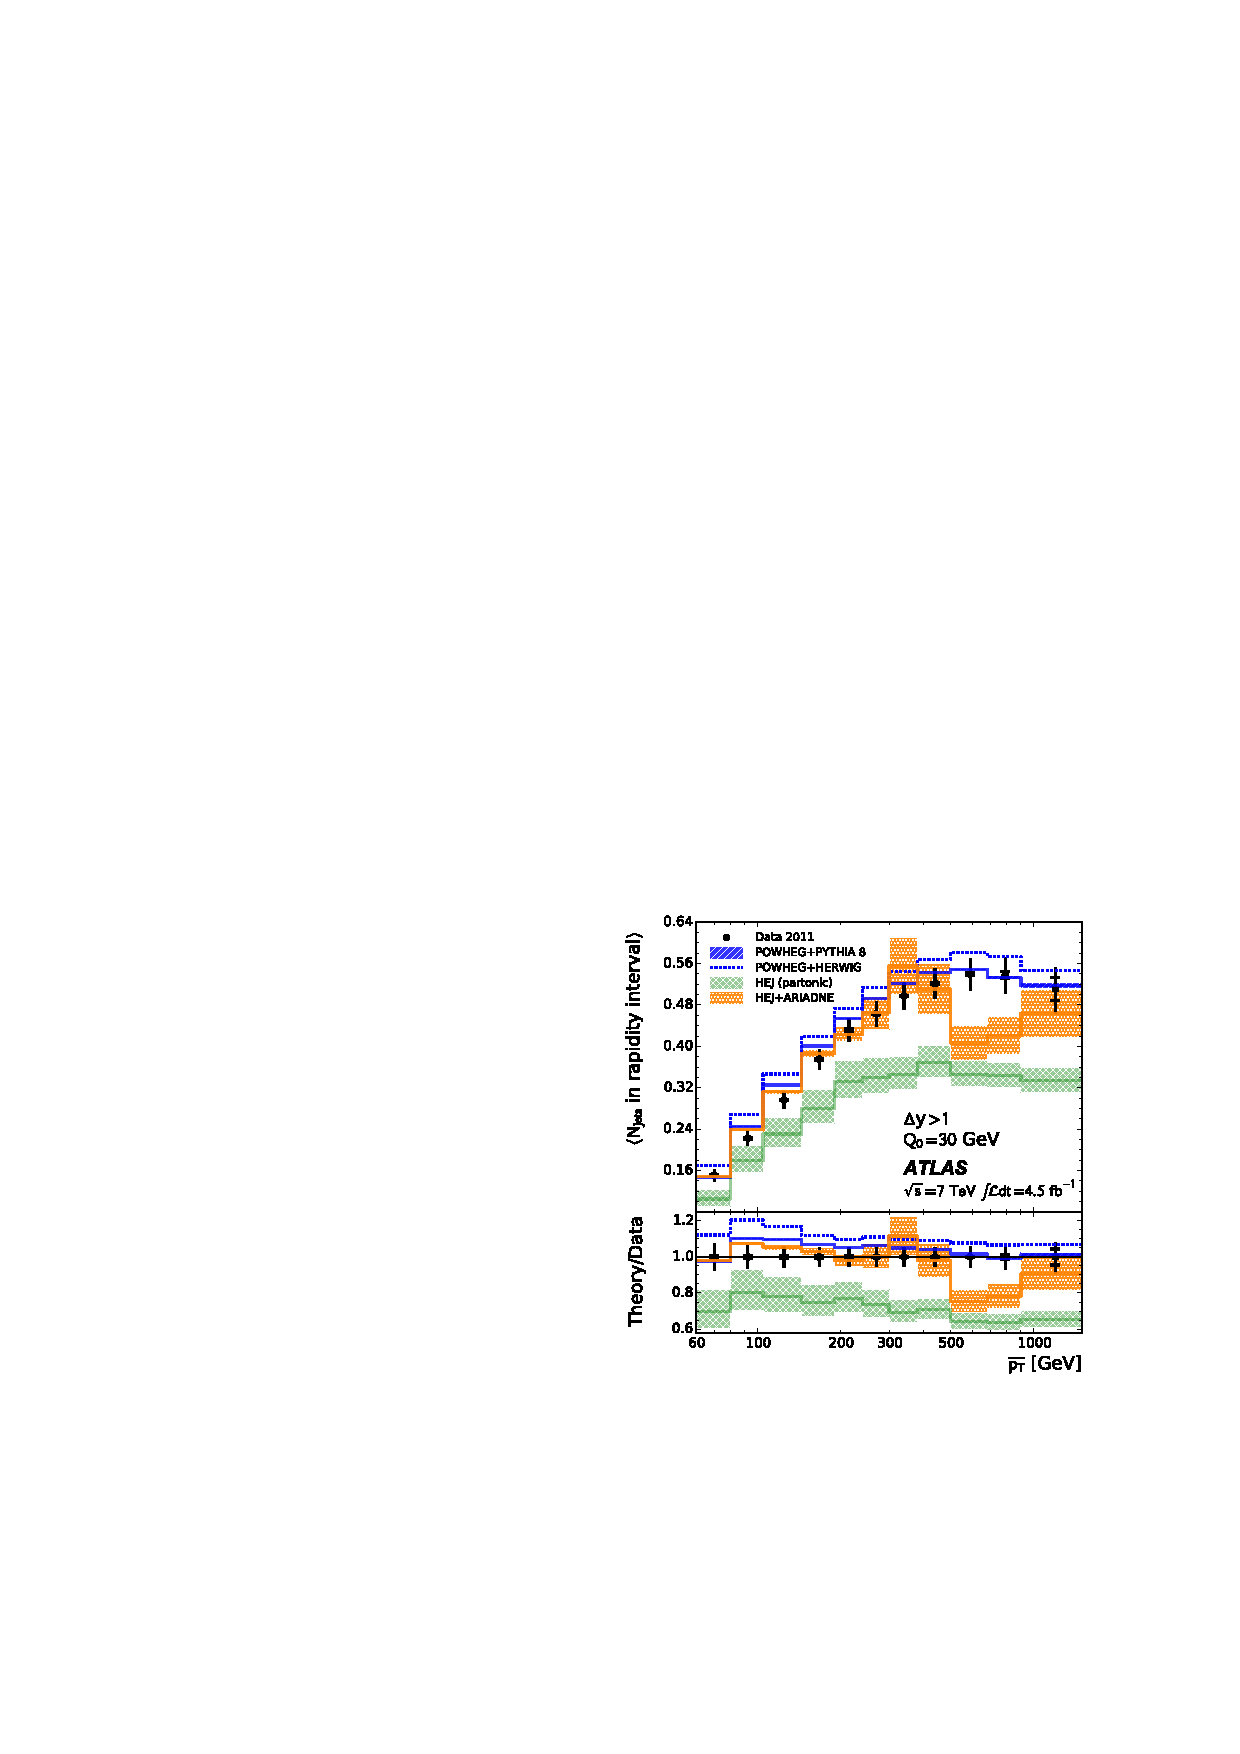
\includegraphics[width=\textwidth, height=1.0\textwidth]{pureJets4b}
			\caption{}
			\label{fig:}
		\end{subfigure}
		\caption{The average number of jets, $\langle N_{\text{jets}}
		\text{ in the rapidity interval}\rangle$, in the rapidity gap
		         bounded by the dijet system, as a function of (a) the
		         rapidity gap, $\Delta y$, and (b) the average $p_T$,
		         $\overline{p_T}$, of the dijet system.}
		\label{fig:atlasPJ2}
	\end{figure}

	We now turn to look at the azimuthal decorrelations of dijet systems.  These are defined
	as $\langle\cos(n(\pi-\Delta\phi))\rangle$ with $n=1, 2, \ldots$.  Here we only consider
	the first and second `moments'; that is, $n=1, 2$.  We follow the notation of \cite{Aad:2014pua}
	and rewrite the second moment as $\langle\cos(2\Delta\phi)\rangle$.  Clearly for a final state
	with two partons momentum conservation will enforce that the jets be in a back-to-back configuration
	i.e. they will have $\Delta \phi=0$ and both $\langle\cos(\pi-\Delta\phi)\rangle$ and
	$\langle\cos(2\Delta\phi)\rangle$ will simply be a flat line $1.0$.  As we allow these hard
	dijets to radiate the moments will depart from the straight line as the constraint softens
	and the extra radiation allows for $\Delta\phi<\pi$.  These moments have long been seen
	as an excellent test of the difference between DGLAP QCD parton showers and BFKL-like
	resummations \cite{Ducloue:2012bm}.  Indeed it is in these figures where we see the biggest
	difference between \HEJ and the \texttt{POWHEG} plus parton shower results.

	Fig.~\eqref{fig:atlasPJ3} shows the first azimuthal moment for the inclusive selection.
	We see that in the 2010 study \HEJA and both \texttt{POWHEG} descriptions slightly
	underestimate $\langle\cos(\pi-\Delta\phi)\rangle$ while the partonic \HEJ result slightly
	overestimates.  However, the evolution of the first azimuthal moment with respect to
	$\overline{p_T}$ shows a clear difference between the two formalisms.  \HEJ does not
	radiate sufficiently to predict the correct decorrelation at low mean transverse momentum
	(which is understood since it does not include the parton shower effects) while both
	\texttt{POWHEG} descriptions cause too much decorrelation at low $\overline{p_T}$.
	The best description of the data is given by \HEJA since it adds extra emissions to High
	Energy Jets which improves our description of the decorrelation.

	\begin{figure}[bth]
		\centering
		\begin{subfigure}[b]{0.48\textwidth}
			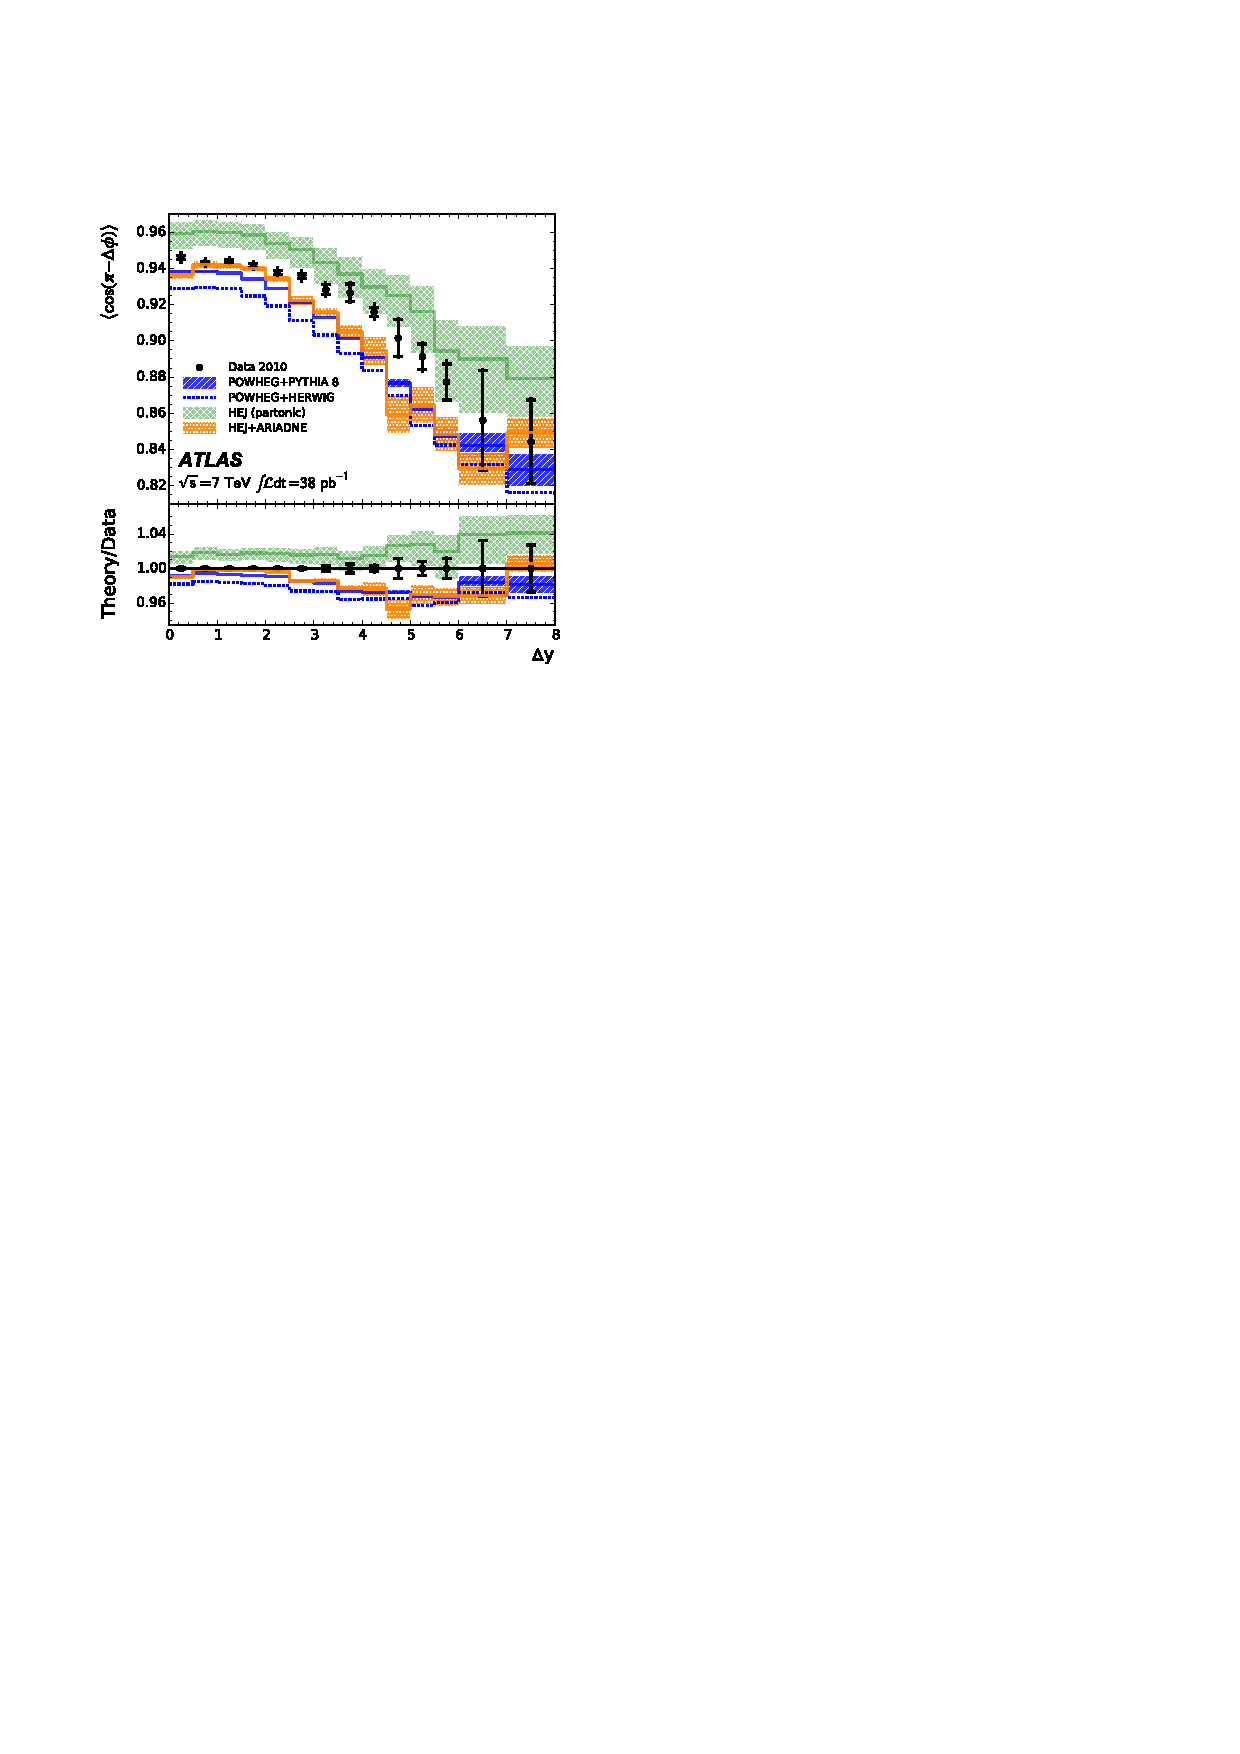
\includegraphics[width=\textwidth, height=1.0\textwidth]{pureJets5a}
			\caption{}
			\label{fig:}
		\end{subfigure}
		~
		\begin{subfigure}[b]{0.48\textwidth}
			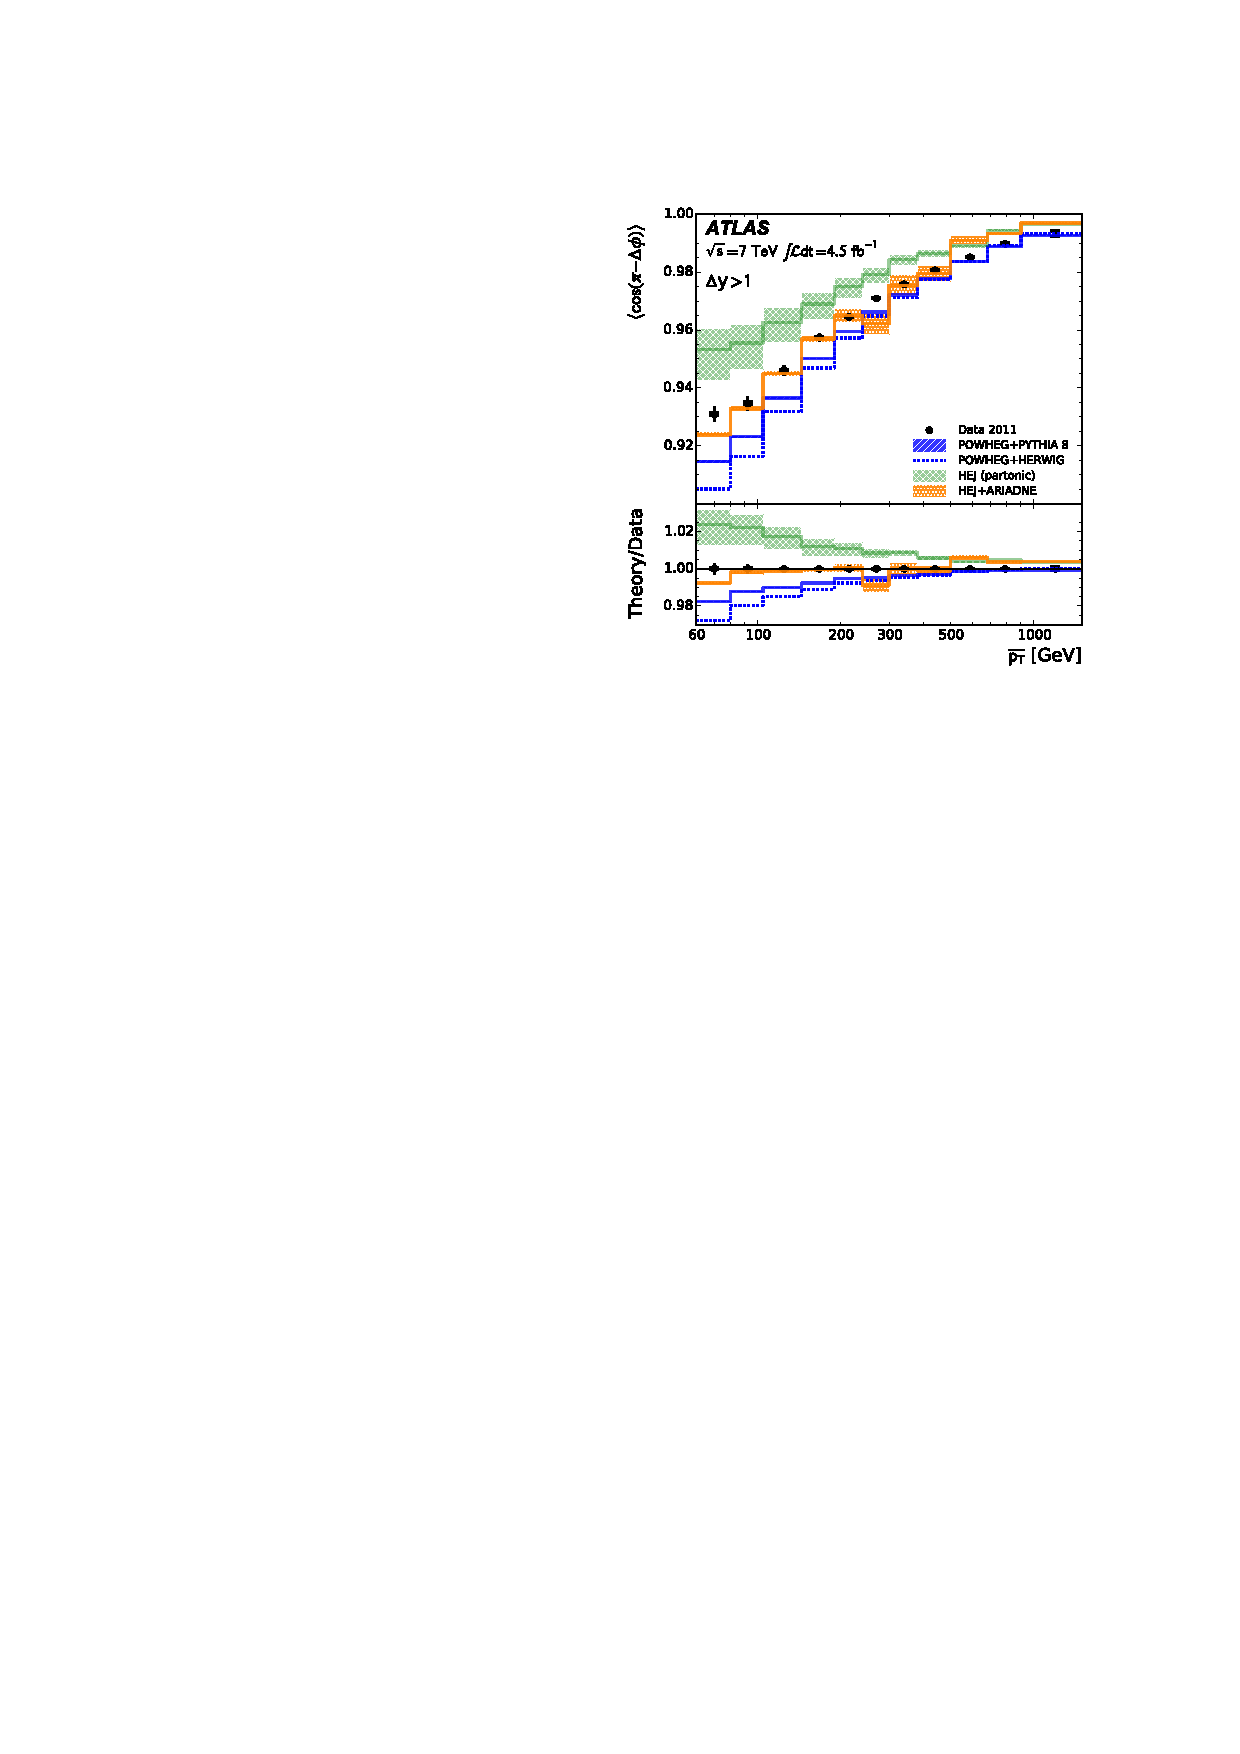
\includegraphics[width=\textwidth, height=1.0\textwidth]{pureJets5b}
			\caption{}
			\label{fig:}
		\end{subfigure}
		\caption{The first azimuthal angular moment, $\langle \cos(\pi-\Delta\phi)\rangle$,
		as a function of (a) the rapidity gap, $\Delta y$ and (b) the average $p_T$,
		$\overline{p_T}$, of the dijet system.}
		\label{fig:atlasPJ3}
	\end{figure}

	Another variable thought to be a good test of DGLAP vs. BFKL physics is the ratio of
	the second moment to the first moment.  This is shown in fig.~\eqref{fig:atlasPJ4}.  Once
	again we do see a sizeable difference in the predictions given by the two resummations.
	Similarly to fig.~\eqref{fig:atlasPJ3} we see that interfacing to the \ARIADNE package
	brings the partonic \HEJ prediction in to a much better agreement of the data.

	\begin{figure}[bth]
		\begin{subfigure}[b]{0.48\textwidth}
			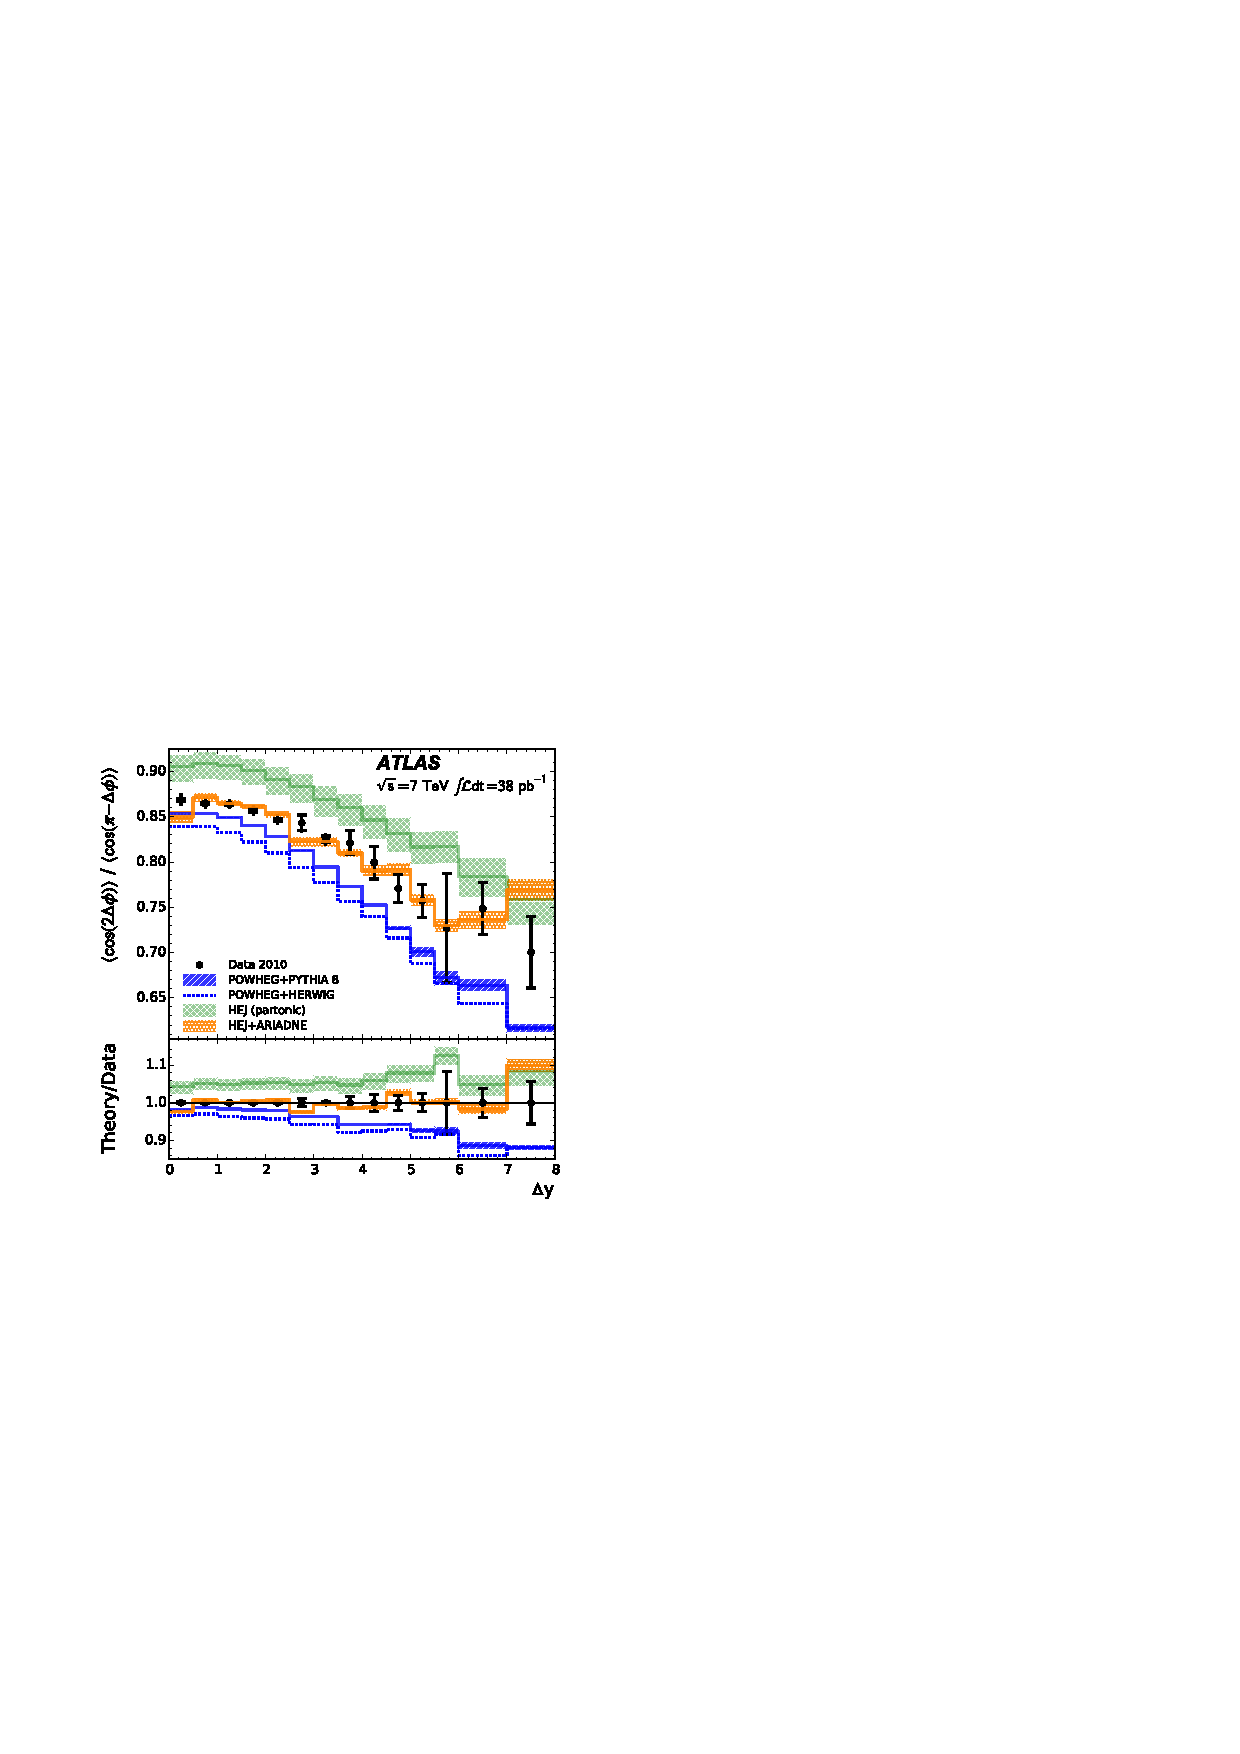
\includegraphics[width=\textwidth, height=1.0\textwidth]{pureJets5c}
			\caption{}
			\label{fig:}
		\end{subfigure}
		~
		\begin{subfigure}[b]{0.48\textwidth}
			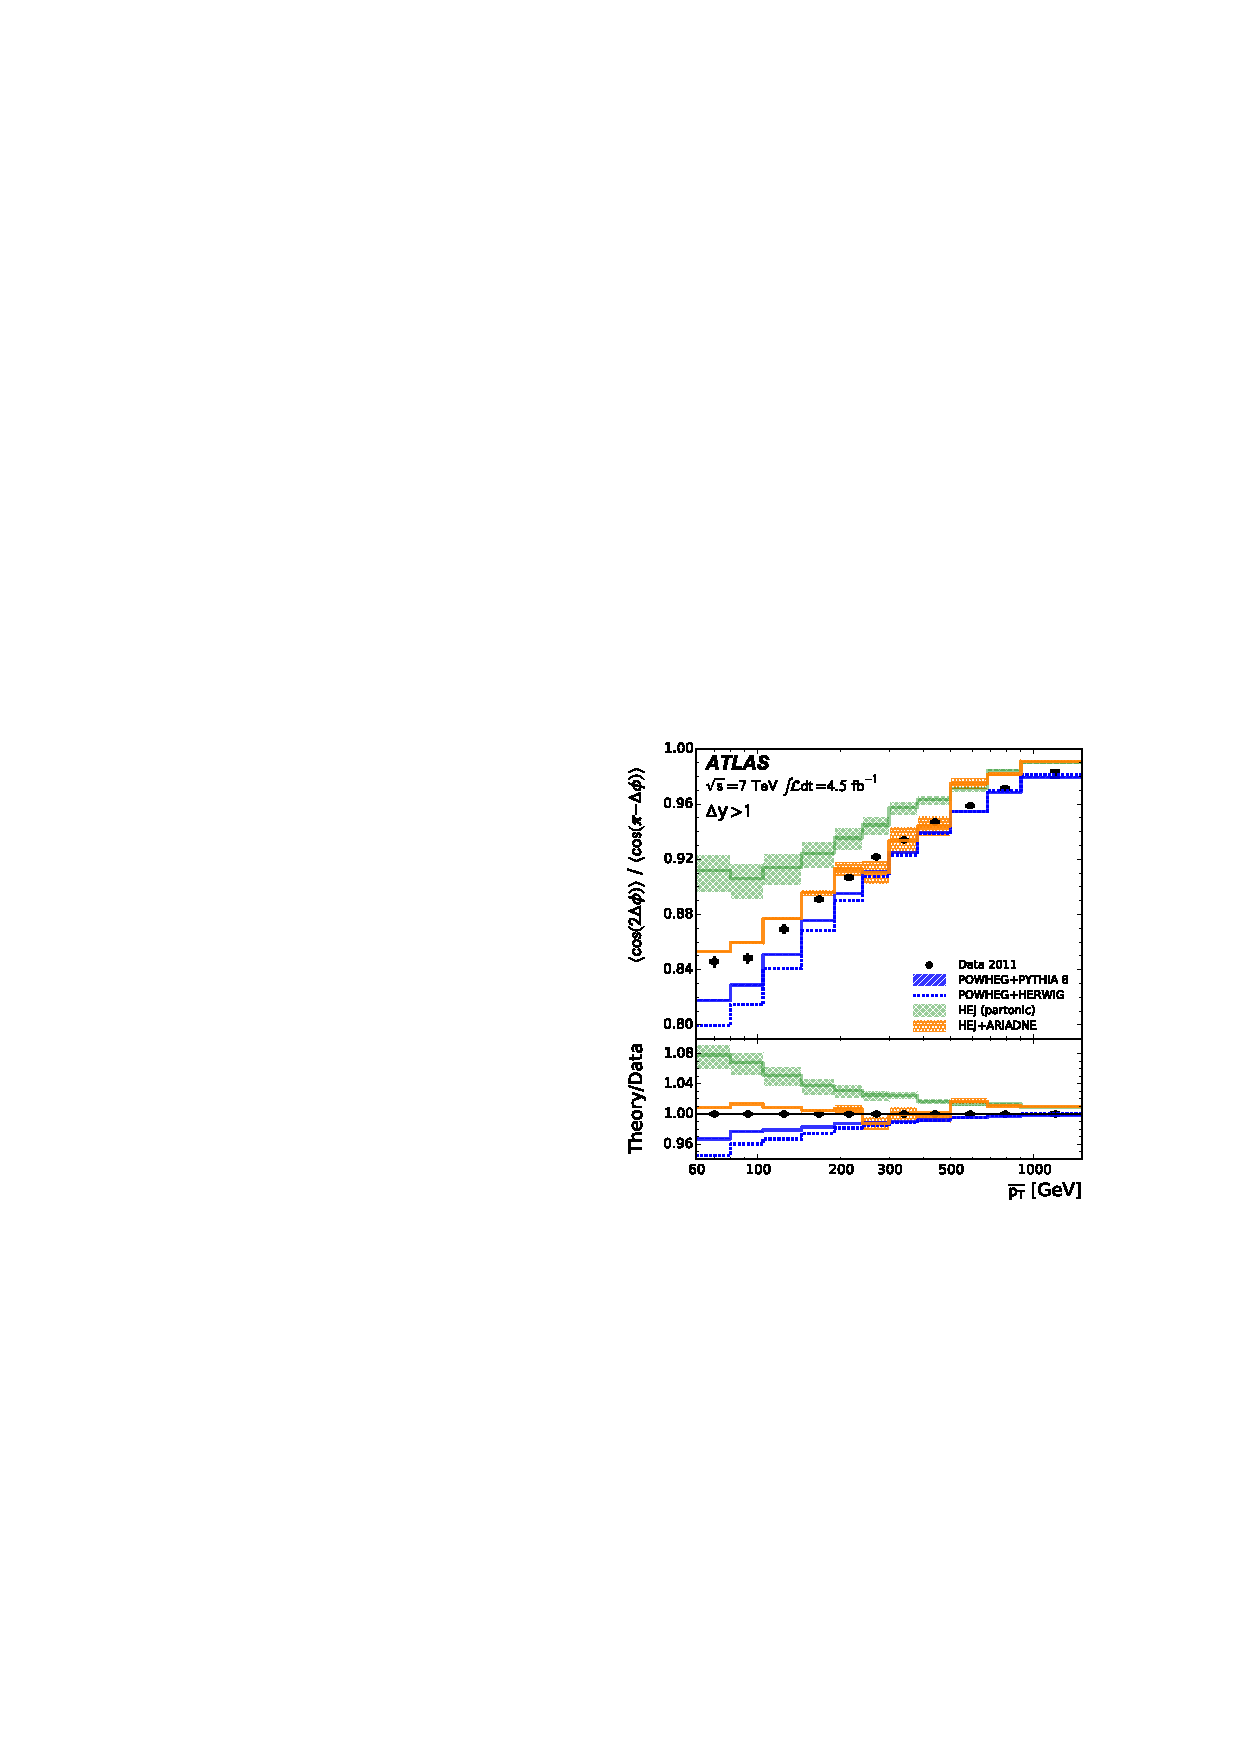
\includegraphics[width=\textwidth, height=1.0\textwidth]{pureJets5d}
			\caption{}
			\label{fig:}
		\end{subfigure}
		\caption{The ratio of the second azimuthal angular moment, $\langle \cos(2\Delta\phi)\rangle$,
		to the first azimuthal angular moment, $\langle \cos(\pi-\Delta\phi)\rangle$, as a function of
		(a) the rapidity gap, $\Delta y$, and (b) the average $p_T$, $\overline{p_T}$, of the dijet system.}
		\label{fig:atlasPJ4}
	\end{figure}

	The two remaining figures are similar to figs. \eqref{fig:atlasPJ3} and \eqref{fig:atlasPJ4} but
	with the addition of the jet veto.  Similarly to the inclusive case we see that the partonic \HEJ
	predictions overestimates the correlation for the 2010 and the 2011 data sets while the NLO plus
	shower predictions, once again, understood the decorrelation.  Given the statistical limited
	data available (especially for the 2010 gap jet vetoed data set) it is more difficult to draw
	clear conclusions here but certainly the inclusion of the \ARIADNE shower improves the High
	Energy Jets results.

	Lastly we have the ratio of the second azimuthal moment to the first azimuthal moment for the
	events which pass the additional jet veto.  \HEJA and \texttt{POWHEG+PYTHIA8} come closest
	to describing the data however there is some disagreement; in particular no one gives a good
	description of the evolution of this ratio at low $\overline{p_T}$.

	In summary, the best description of the data overall is given by \HEJA and \texttt{POWHEG+PYTHIA8}
	while parton level \HEJ overestimates (underestimate) the gap fraction (the mean number of jets
	in the rapidity gap bounded between the dijet system) and overshoots both the first azimuthal
	moment and the ratio of the second to the first azimuthal moment.  \texttt{POWHEG+HERWIG} describes
	the data poorly for the gap fraction, the mean number of gap jets and the azimuthal decorrelations.
	From this it is clear that while the logarithmically enhanced resummed in the High Energy Jets
	framework are important in regions of phase space where we have large rapidity gaps (such as the
	analyses described here) there are equally important contributions arising from the logarithms
	given to us by the interface with a parton shower.

	\begin{figure}[bth]
		\centering
		\begin{subfigure}[b]{0.48\textwidth}
			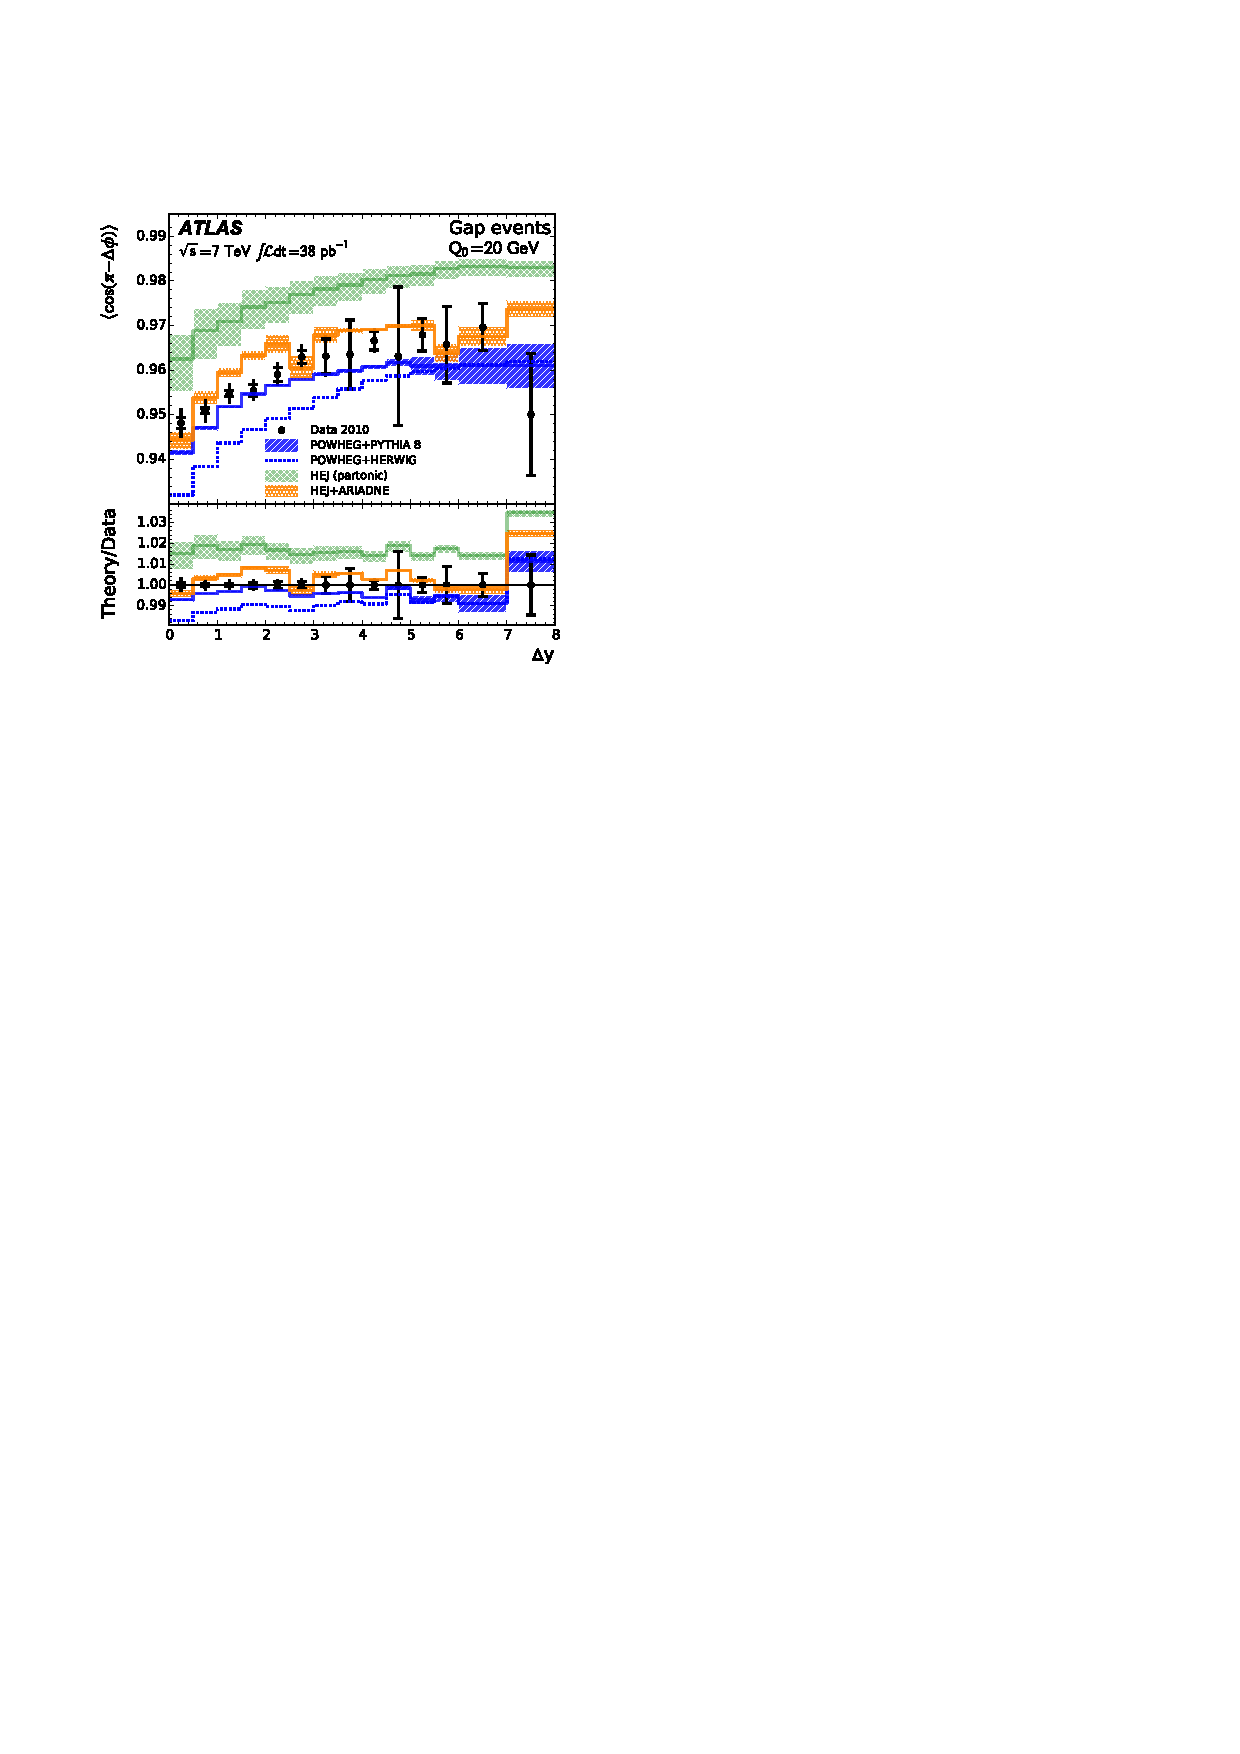
\includegraphics[width=\textwidth, height=1.0\textwidth]{pureJets6a}
			\caption{}
			\label{fig:}
		\end{subfigure}
		~
		\begin{subfigure}[b]{0.48\textwidth}
			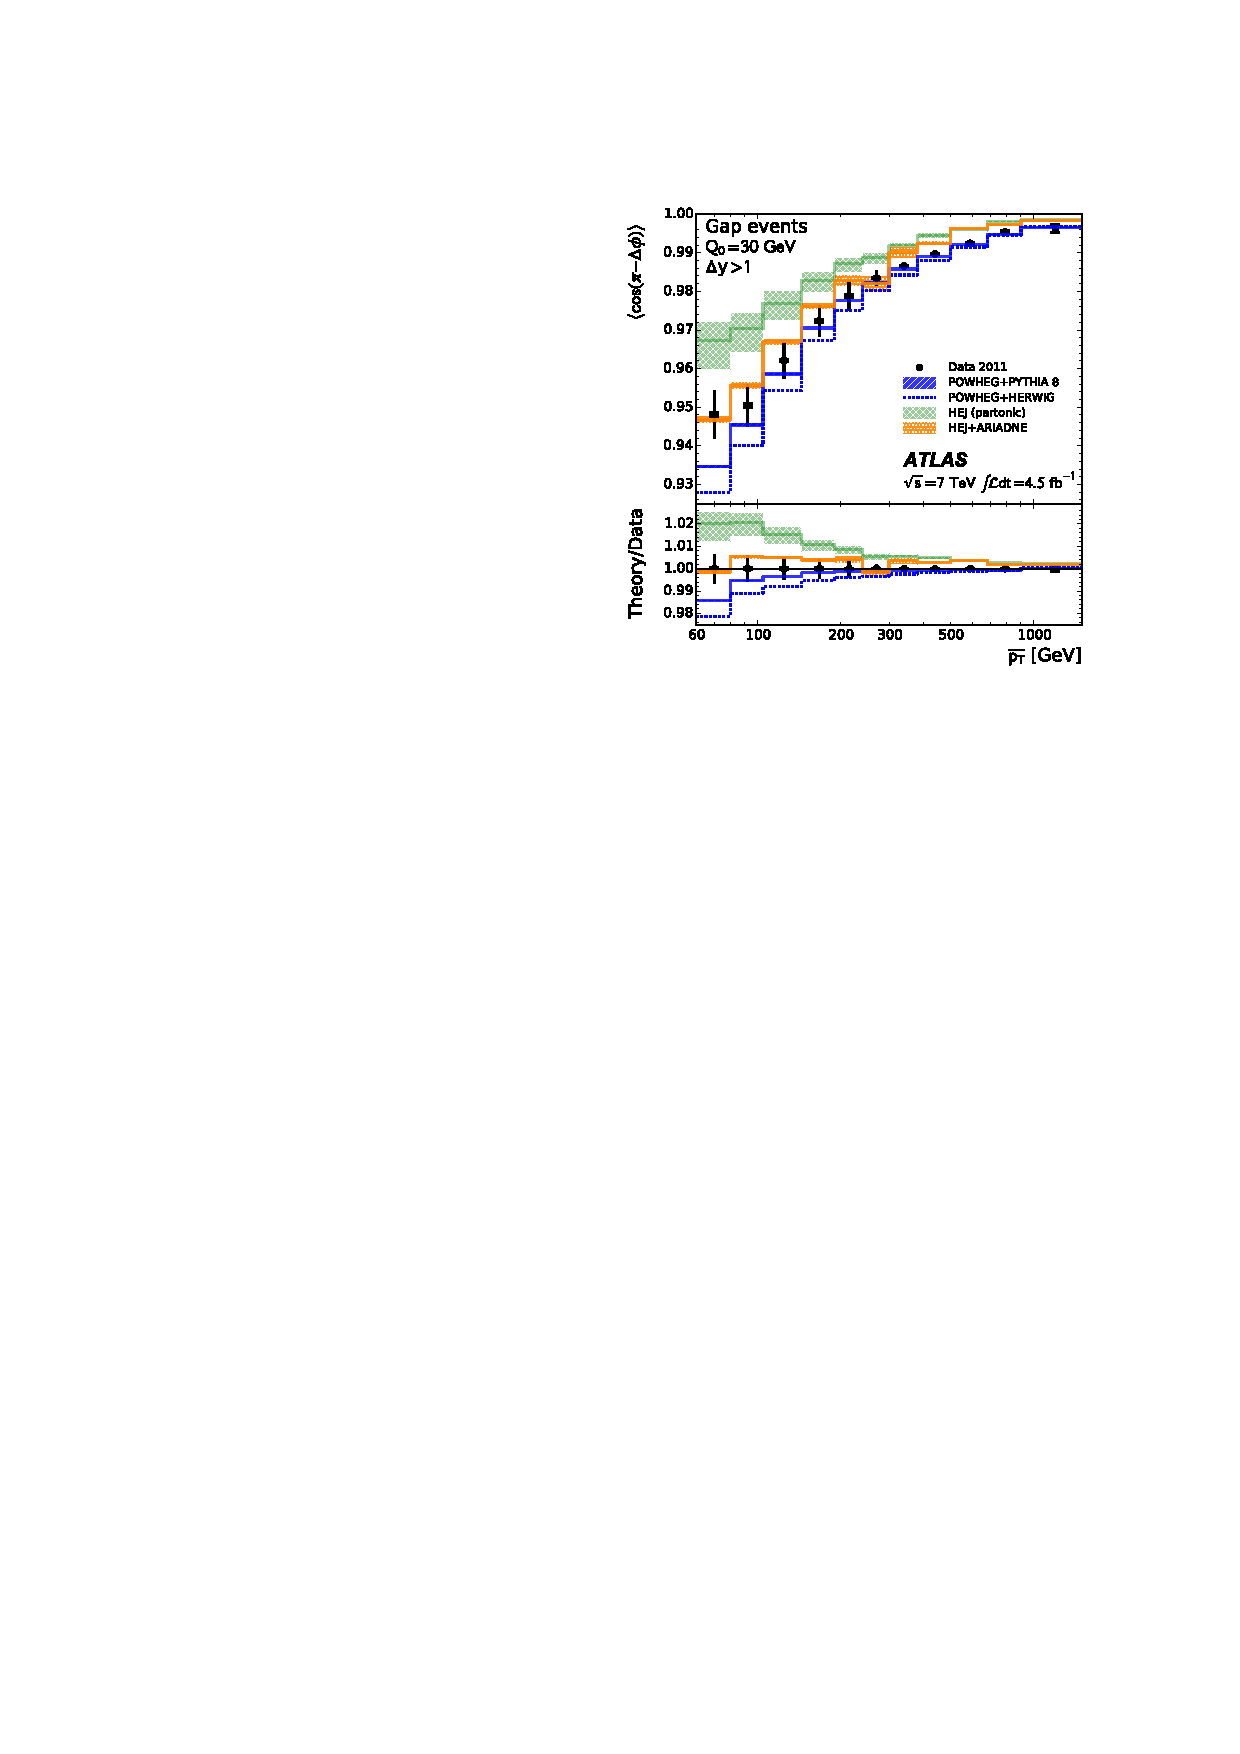
\includegraphics[width=\textwidth, height=1.0\textwidth]{pureJets6b}
			\caption{}
			\label{fig:}
		\end{subfigure}
		\caption{The first azimuthal angular moment, $\langle \cos(\pi-\Delta\phi)\rangle$,
		for events passing the veto on gap activity above $Q_0=20\text{GeV}$ as a function
		of (a) the rapidity gap, $\Delta y$, and (b) the average $p_T$, $\overline{p_T}$,
		of the dijet system.}
		\label{fig:atlasPJ5}
	\end{figure}

	\begin{figure}[bth]
		\begin{subfigure}[b]{0.48\textwidth}
			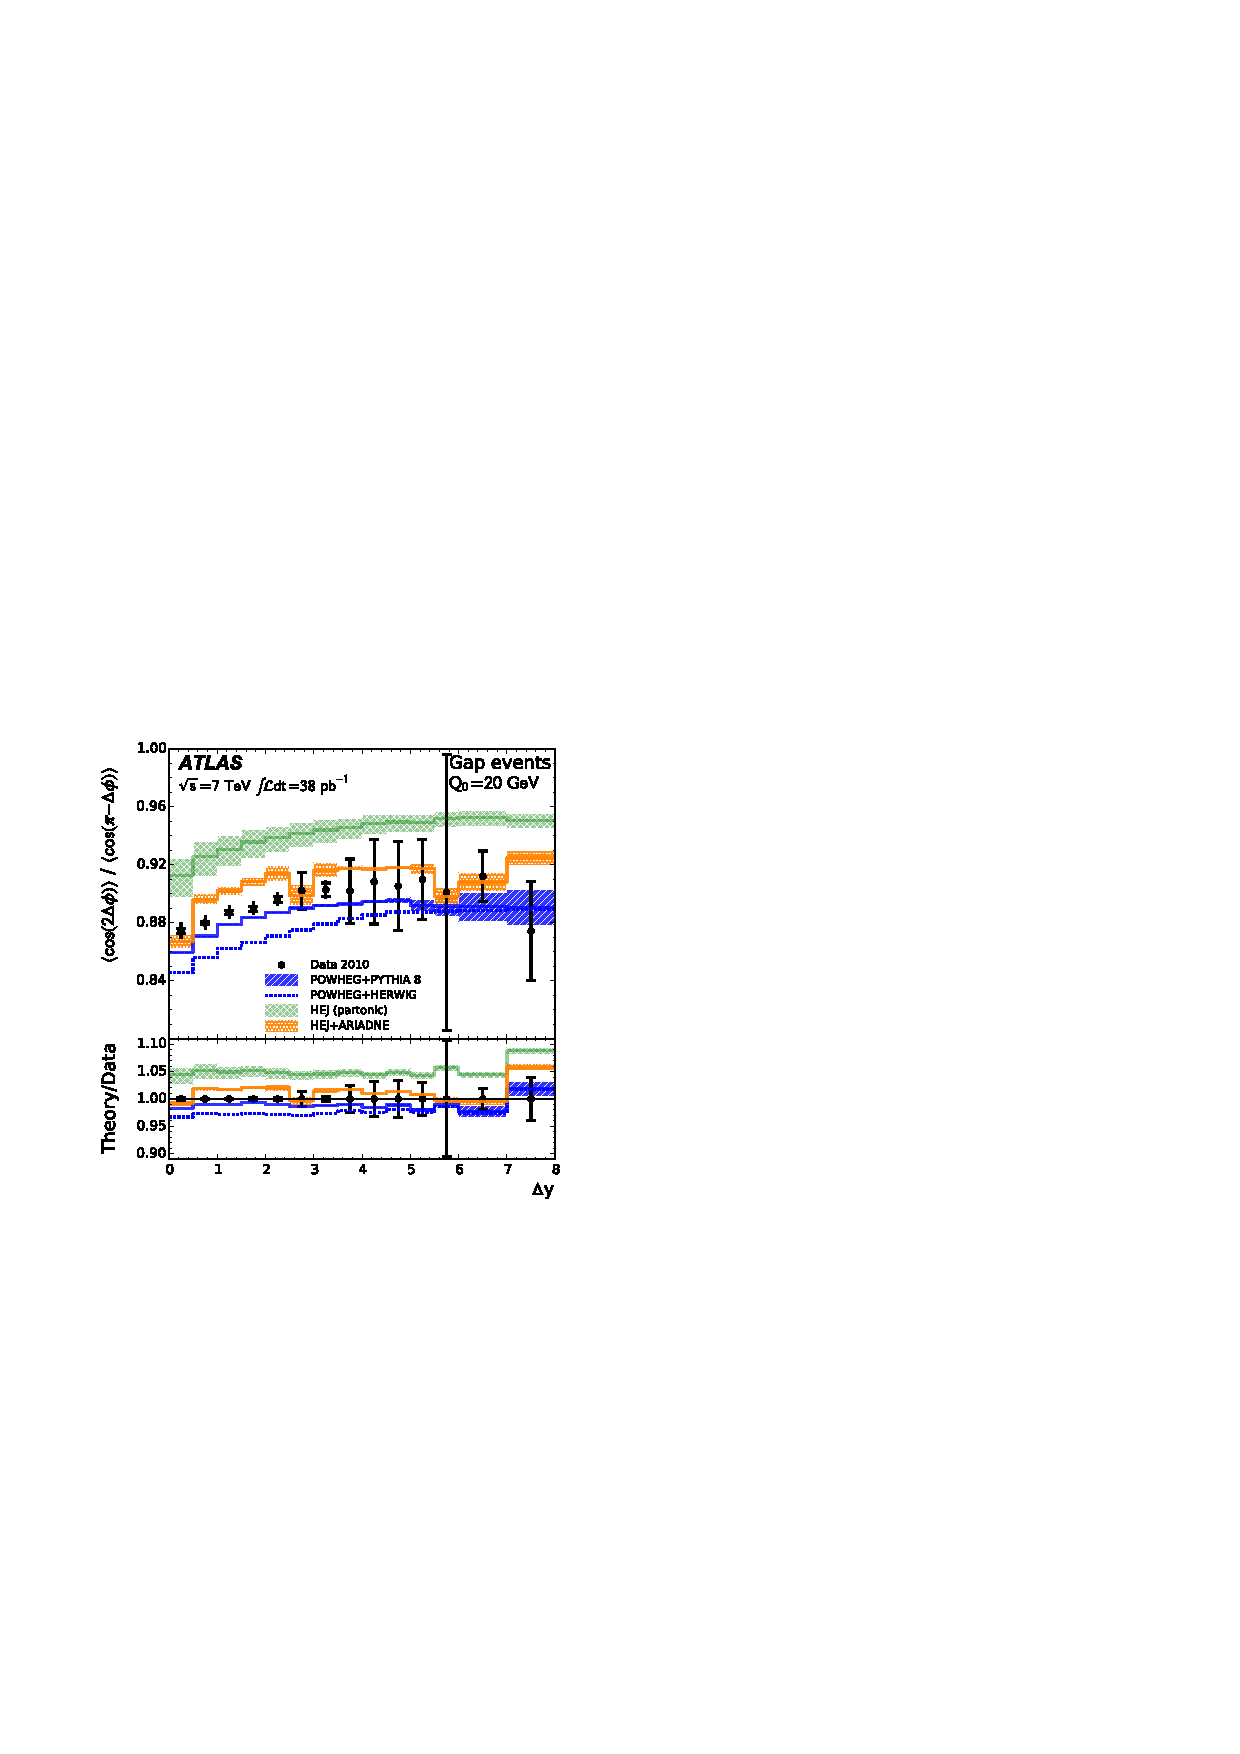
\includegraphics[width=\textwidth, height=1.0\textwidth]{pureJets6c}
			\caption{}
			\label{fig:}
		\end{subfigure}
		~
		\begin{subfigure}[b]{0.48\textwidth}
			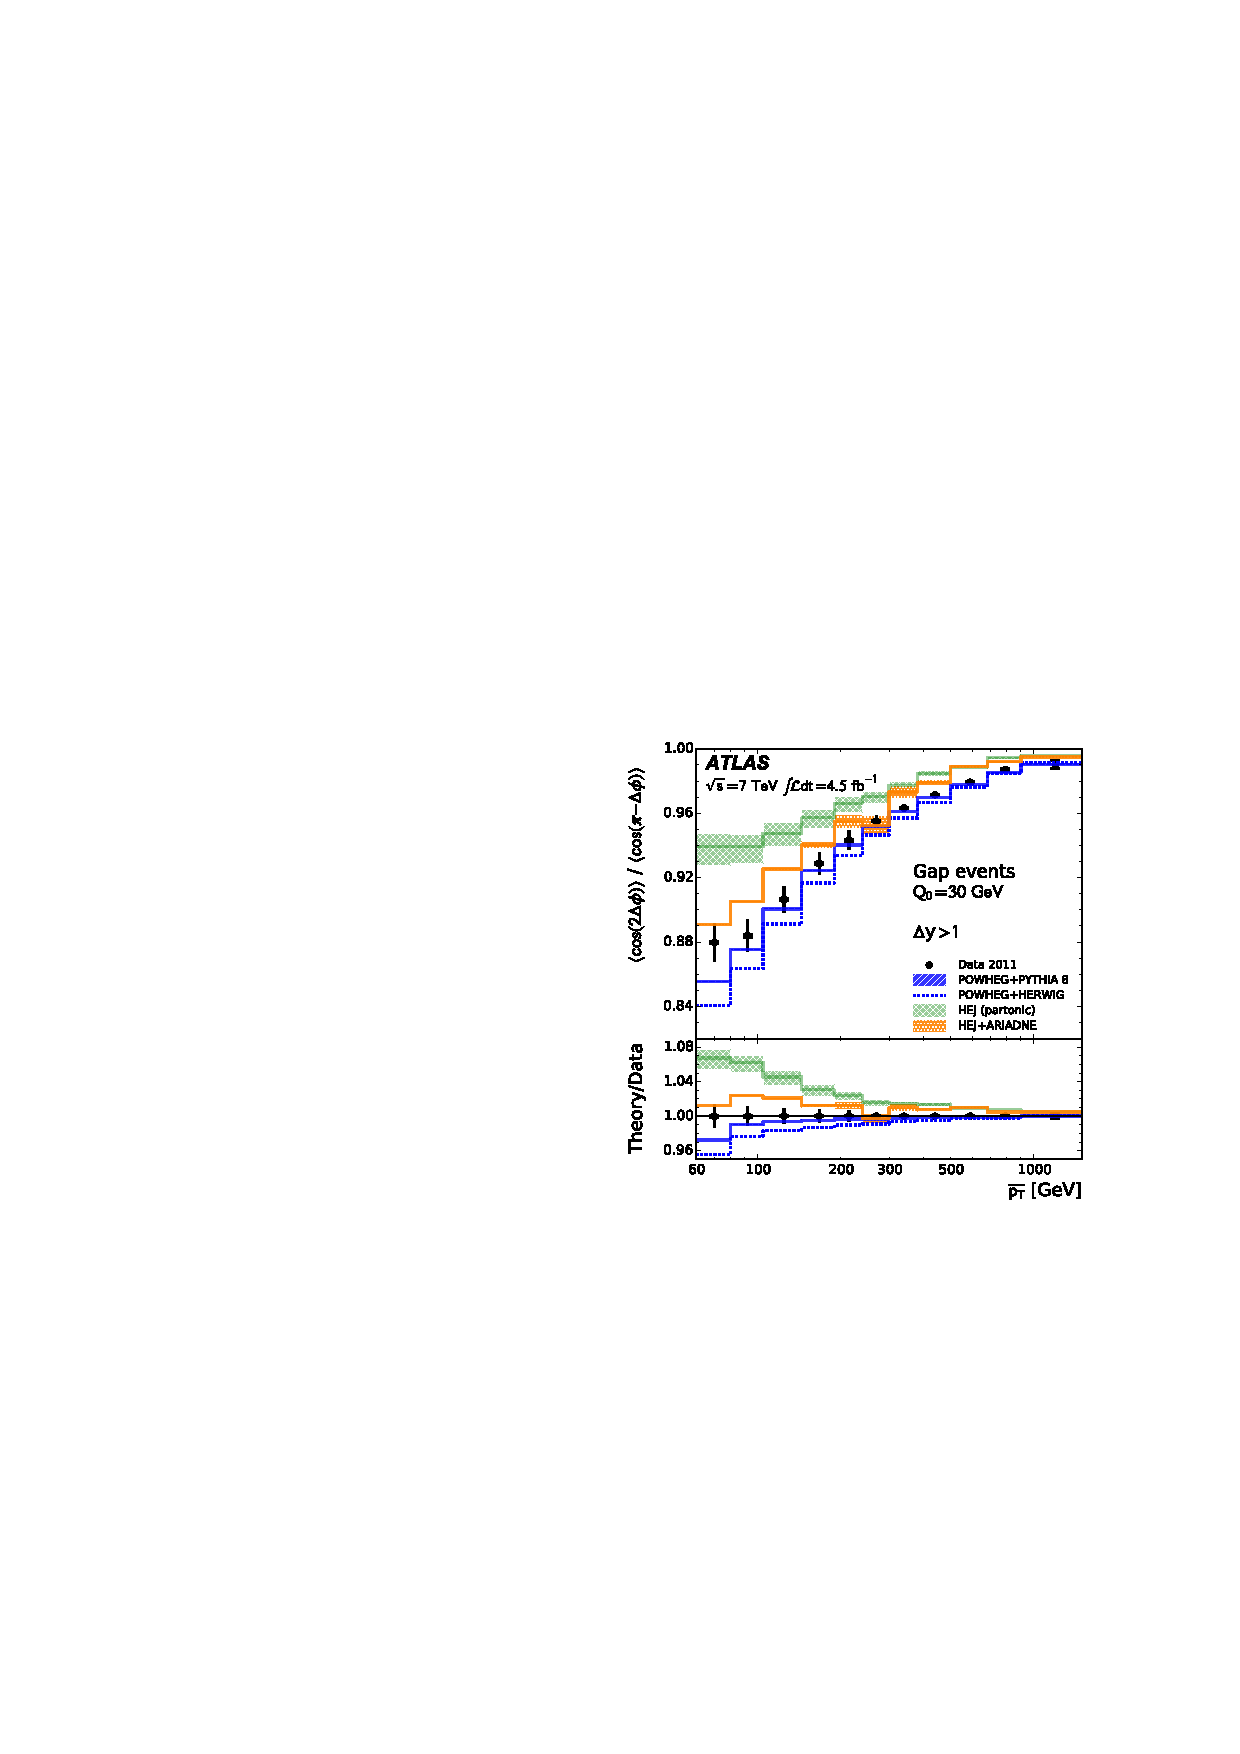
\includegraphics[width=\textwidth, height=1.0\textwidth]{pureJets6d}
			\caption{}
			\label{fig:}
		\end{subfigure}
		\caption{The ratio of the second azimuthal angular moment,
		$\langle \cos(2\Delta\phi)\rangle$, to the first azimuthal angular moment,
		$\langle \cos(\pi-\Delta\phi)\rangle$, as a function of (a) the rapidity gap,
		$\Delta y$, and (b) the average $p_T$, $\overline{p_T}$, of the dijet system.  A
		veto of $Q_0=20\text{GeV}$, for (a), and $Q_0=30\text{GeV}$, for (b), is applied
		on activity in the rapidity gap is applied.}
		\label{fig:atlasPJ6}
	\end{figure}

\chapter{$\zg$+Jets at 100TeV}
\label{chap:100TeV}

	\begin{itemize}
		\item Talk about the FCC movement and the effect we expect the resummation will have at these energies.
		\item Put all three lines (30GeV, 60GeV, 100GeV) on the same plots in this section?
		\item Pros: Can see that we can put more stringent cuts while maintaining x-section.  Also
		      makes the point that we can cut out all the NP physics we cant model.
		\item Cons: Plots will be very busy.
	\end{itemize}

	Even as the Large Hadron Collider was beginning its first run people were thinking about the next machine
	We now discuss the results of

	\begin{figure}[h]
		\centering
		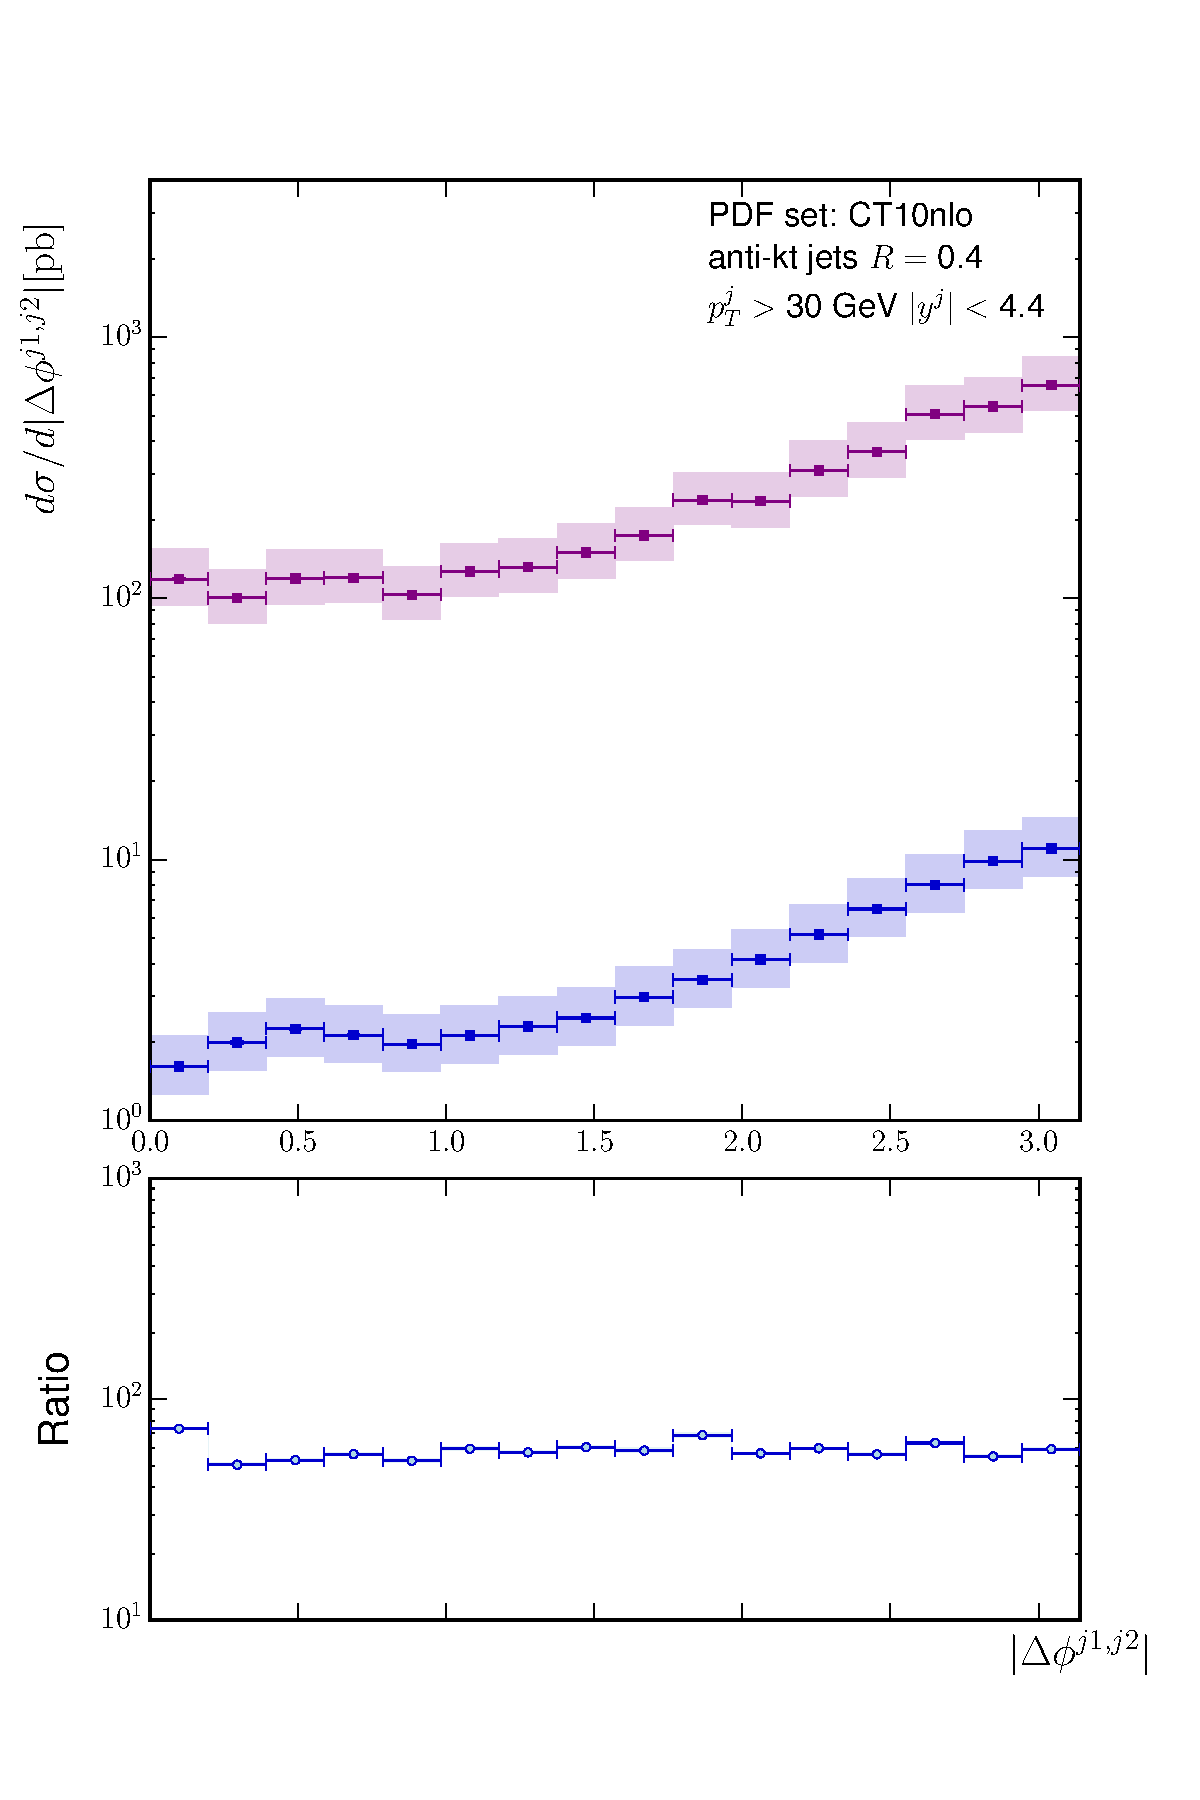
\includegraphics[width=0.8\linewidth]{ATLAS_Z_100TeV_12a}
		\caption{The differential cross-section for $\zg$ plus inclusive dijets as a
		function of the azimuthal separation of the dijet system shown for centre-of-mass
		energies of 7TeV (blue) and 100TeV (pink).}
		\label{fig:100tev_12a}
	\end{figure}

	Fig. (\eqref{fig:100tev_12a}) notes:

	\begin{itemize}
		\item dphi plot
		\item Start with this one because its the most boring,
		\item i.e. if QCD didnt change with energy scale all plots would be like this one
	\end{itemize}

	\begin{figure}[h]
		\centering
		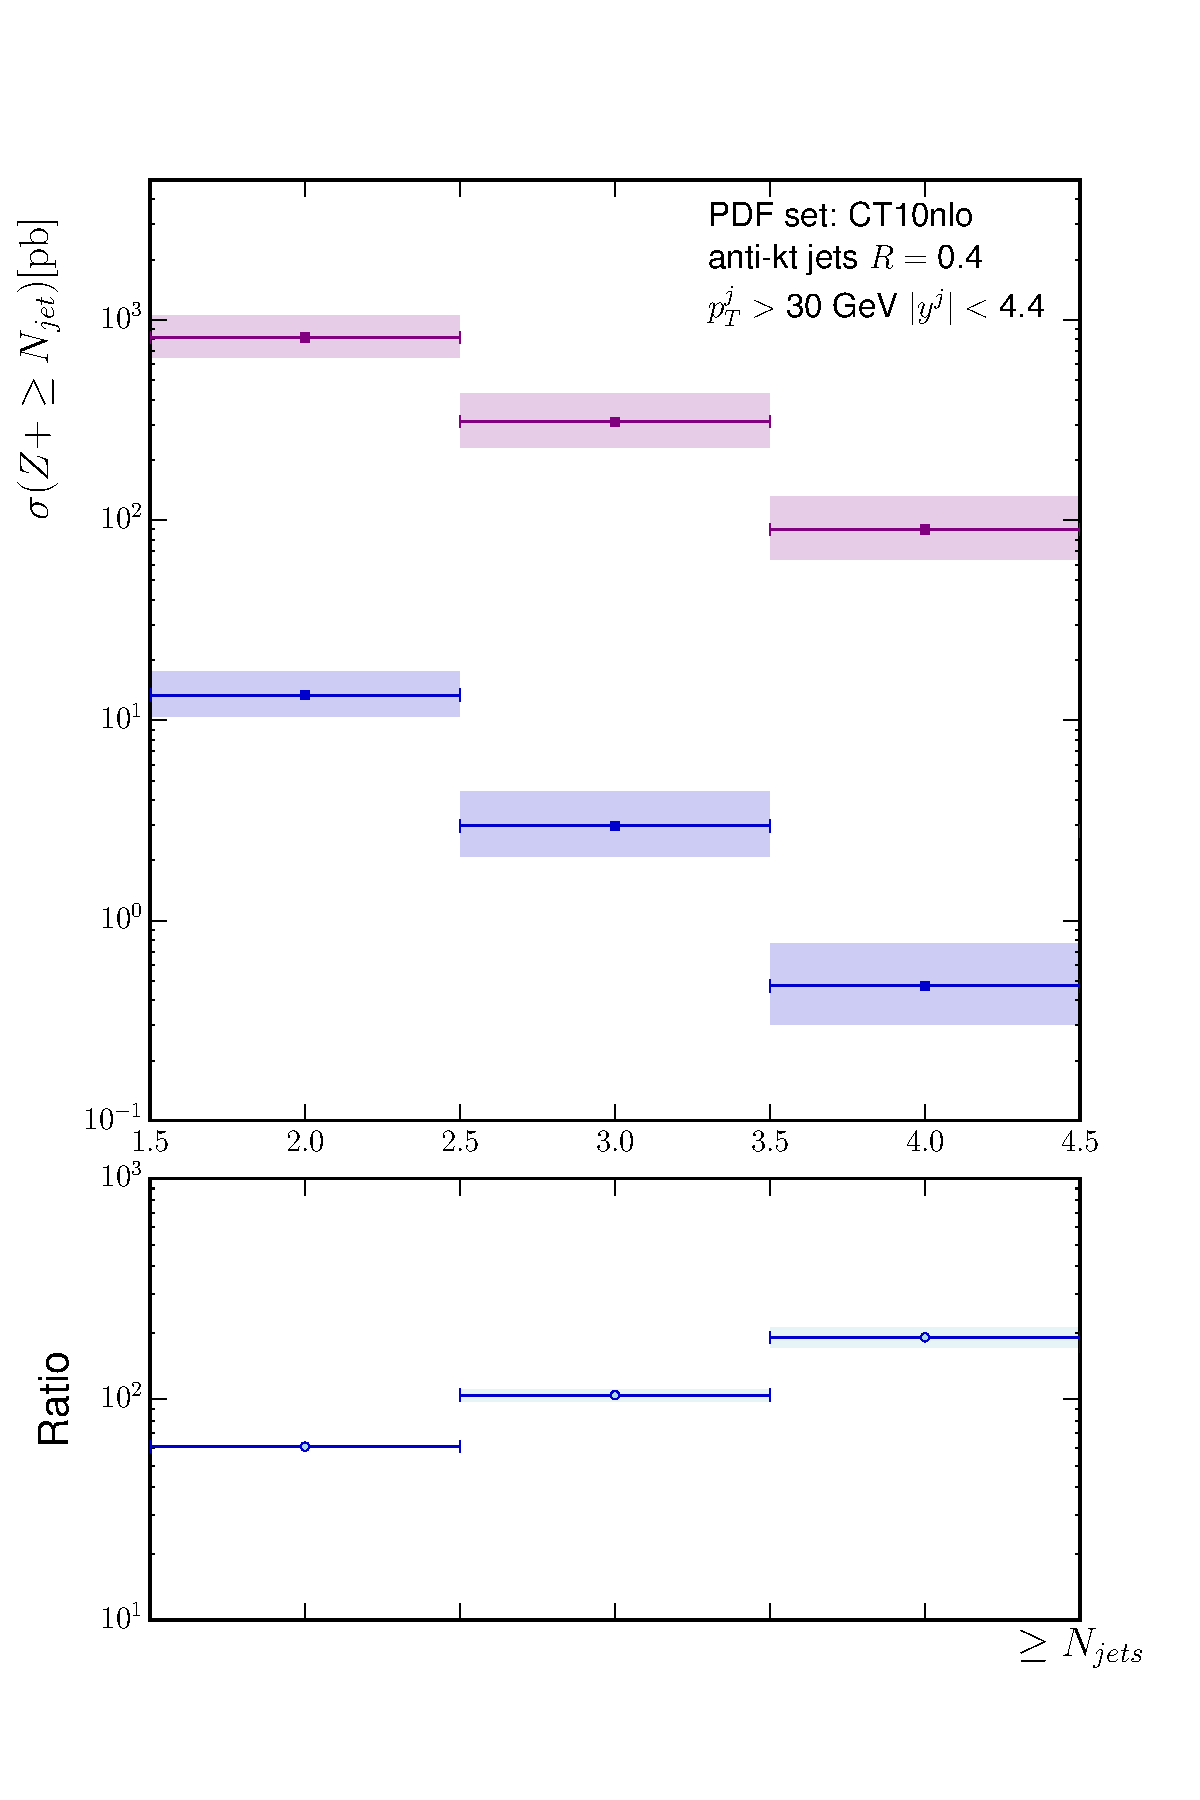
\includegraphics[width=0.8\linewidth]{ATLAS_Z_100TeV_2a}
		\caption{The cross-section for $\zg$ plus inclusive dijets as a function of the number of jets $N_{\text{jet}}$ shown for
		         centre-of-mass energies of 7TeV (blue) and 100TeV (pink).}
		\label{fig:100tev_2a}
	\end{figure}

	Fig. (\eqref{fig:100tev_2a}) notes:

	\begin{itemize}
		\item njets,
		\item Explicitly shows that the break-down of the perturbative series gets worse at higher energies,
		\item The contributions from higher-order corrections increase as the energy increases,
	\end{itemize}

	\begin{figure}[h]
		\centering
		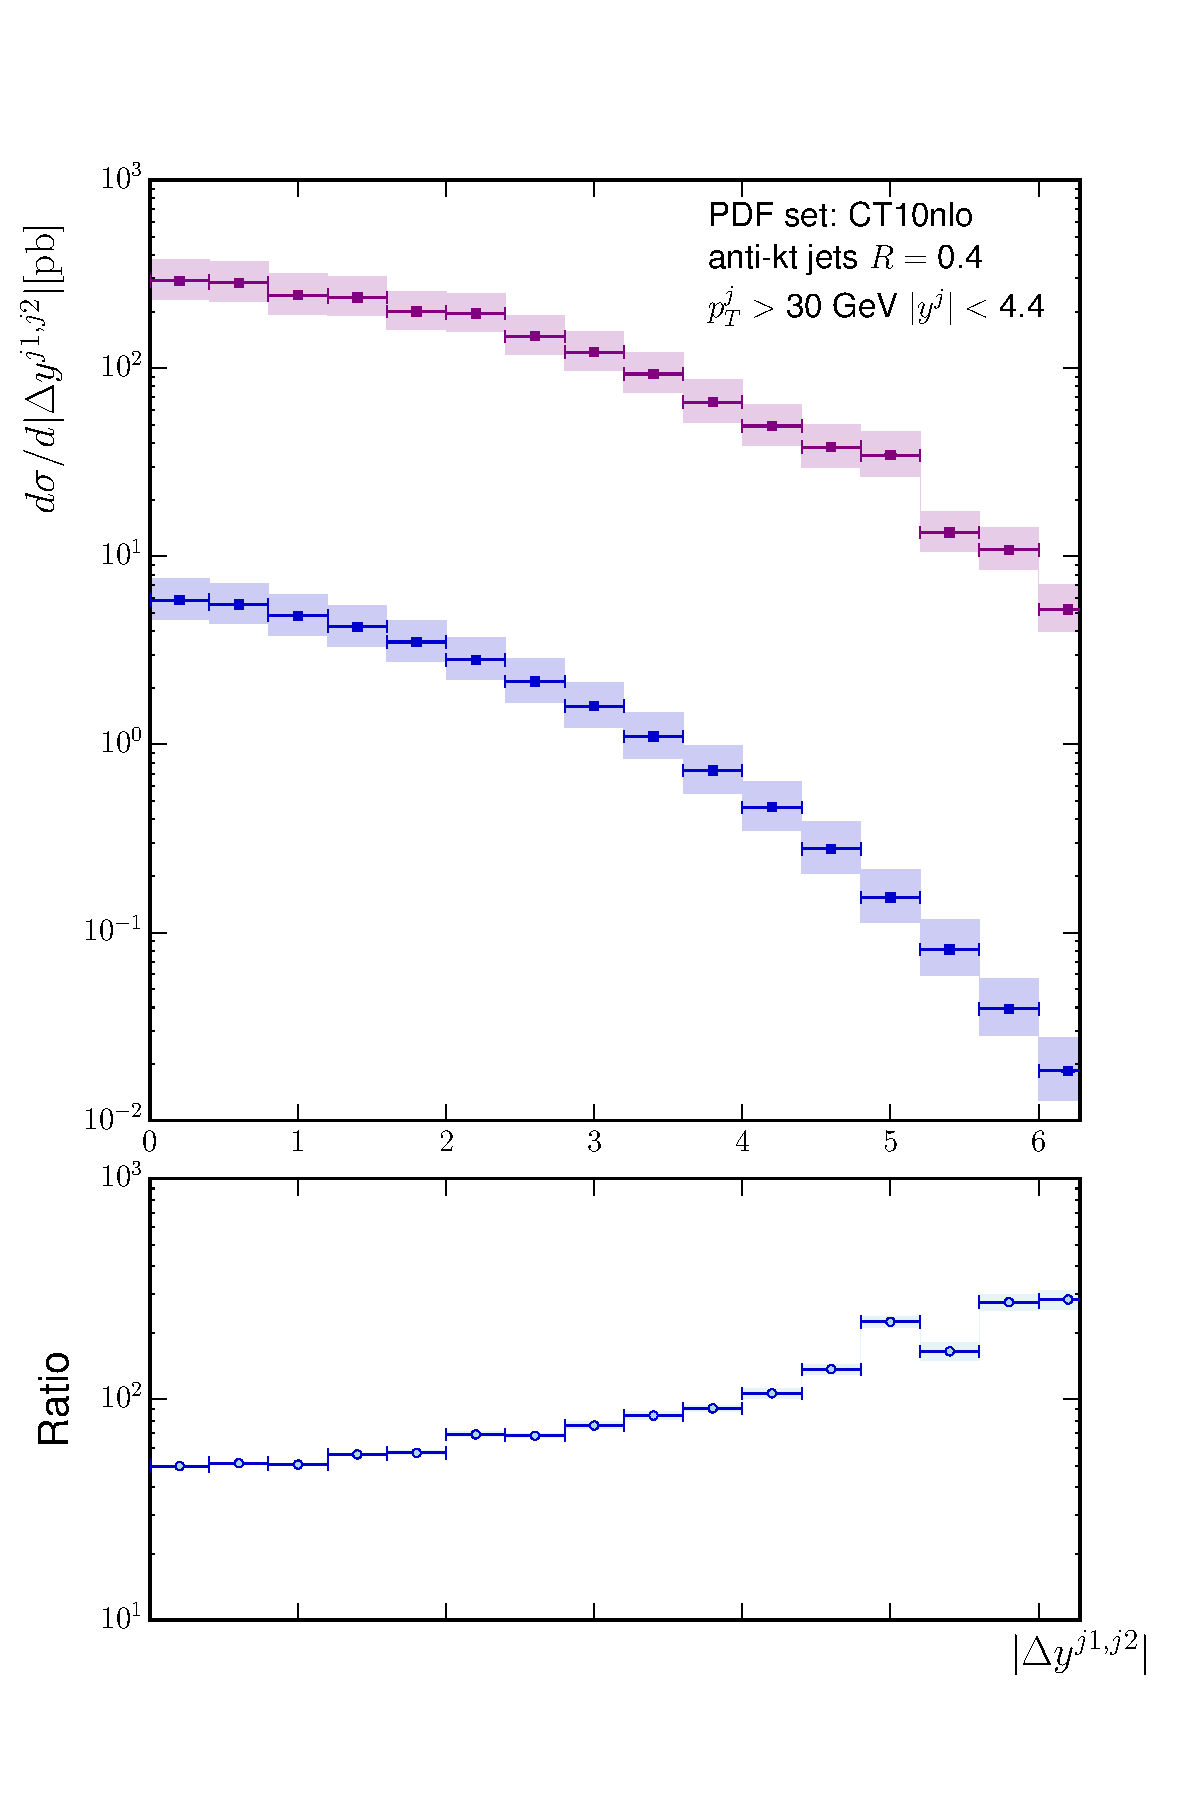
\includegraphics[width=0.8\linewidth]{ATLAS_Z_100TeV_11a}
		\caption{The differential cross-section for $\zg$ plus inclusive dijets as a function of the absolute value of the
		         rapidity gap between the dijets, $\Delta y^{j1, j2}$ shown for centre-of-mass energies of 7TeV (blue) and
		         100TeV (pink).}
		\label{fig:100tev_11a}
	\end{figure}

	Fig. (\eqref{fig:100tev_11a}) notes:

	\begin{itemize}
		\item dy plot,
		\item O(10) increase in cross-section as we go to large rapidities,
		\item More energy in initial state means we can get more jets further in to the outer regions of y-space,
		\item The increase seen is \emph{exactly} the large logs we capture at play
	\end{itemize}

	\begin{figure}[h]
		\centering
		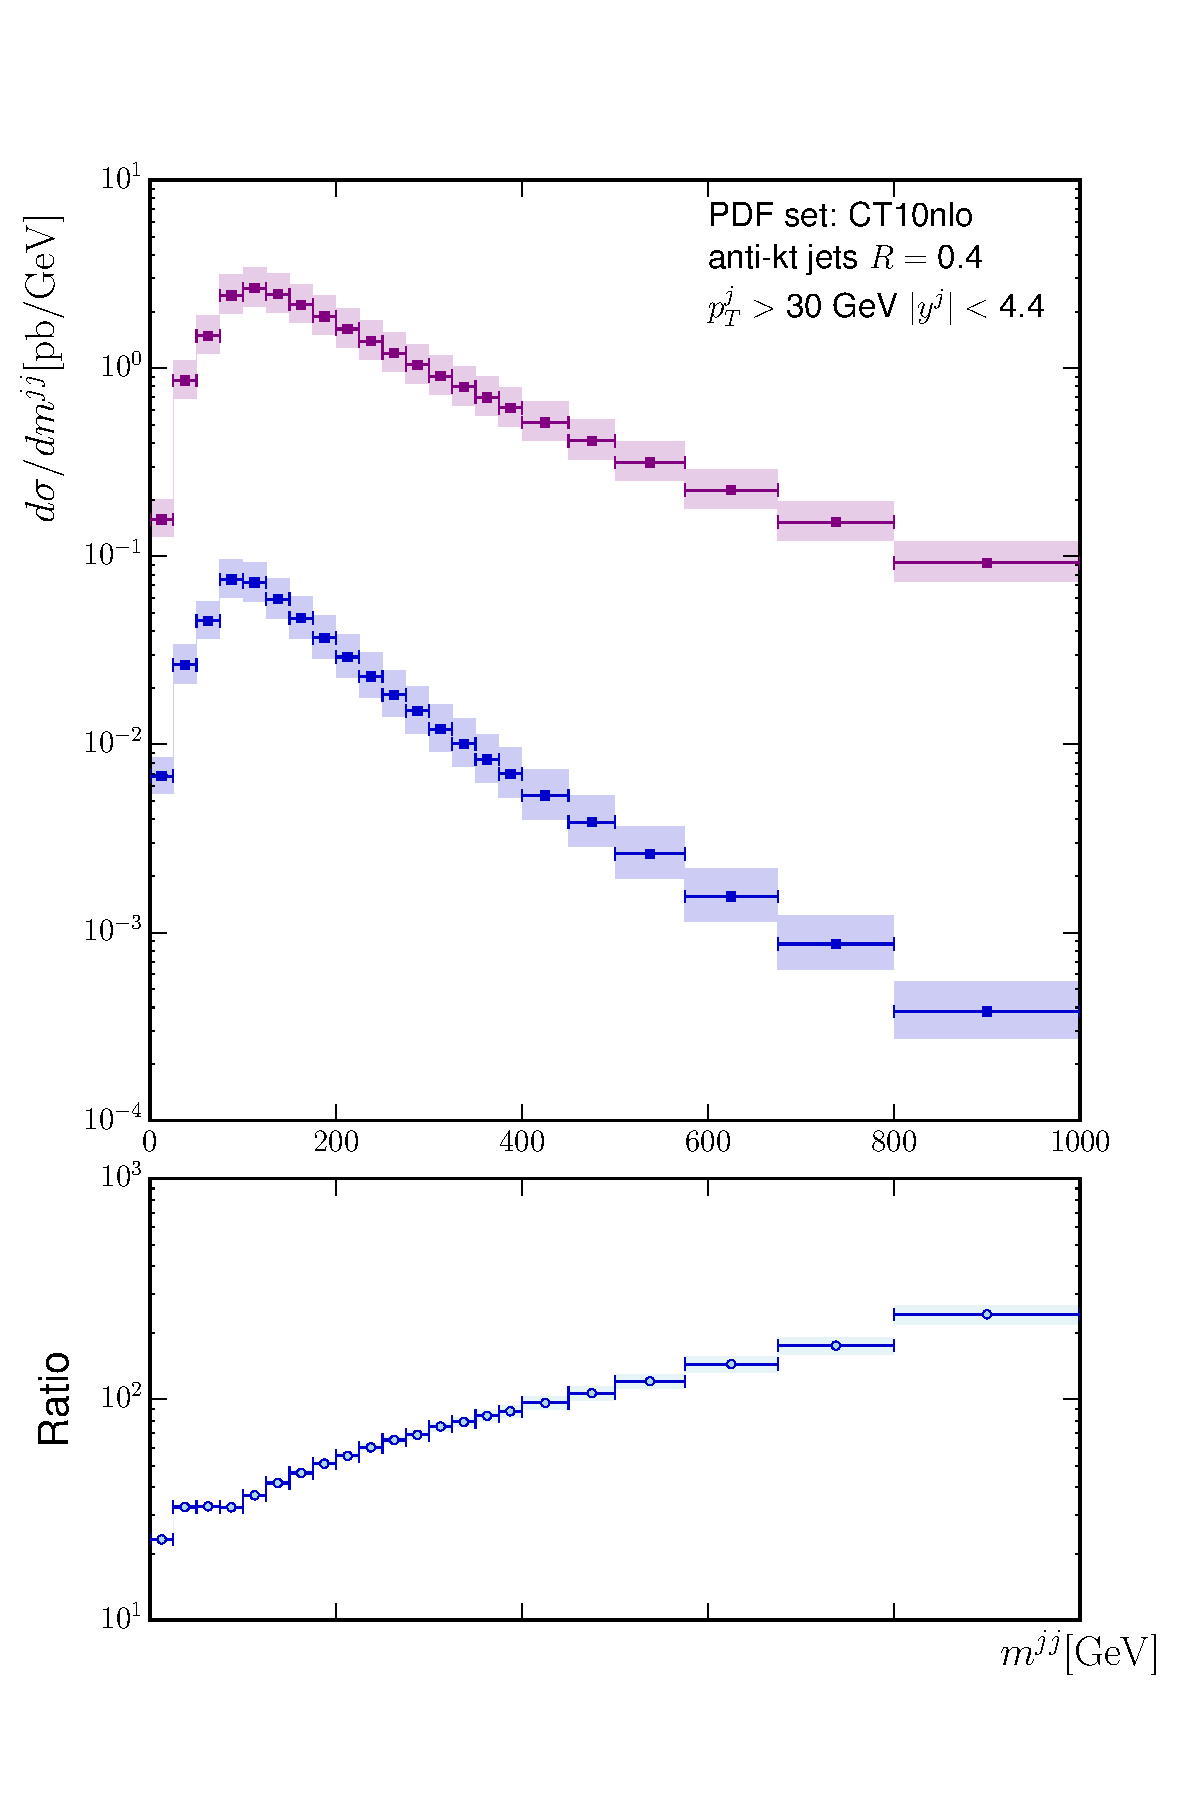
\includegraphics[width=0.8\linewidth]{ATLAS_Z_100TeV_11b}
		\caption{The differential cross-section for $\zg$ plus inclusive dijets as a function of the invariant mass
		         of the dijets, $m^{jj}$, shown for centre-of-mass energies of 7TeV (blue) and 100TeV (pink).}
		\label{fig:100tev_11b}
	\end{figure}

	Fig. (\eqref{fig:100tev_11b}) notes:

	\begin{itemize}
		\item $dm_jj$ plot,
		\item O(10) increase in cross-section as we go to large invariant masses,
		\item Invariant masses again correlate with the logs we resum (show this explicitly if you havent already),
		\item Similar to fig. (\eqref{fig:100tev_11a})
	\end{itemize}

	\begin{figure}[h]
		\centering
		\begin{subfigure}[b]{0.48\textwidth}
			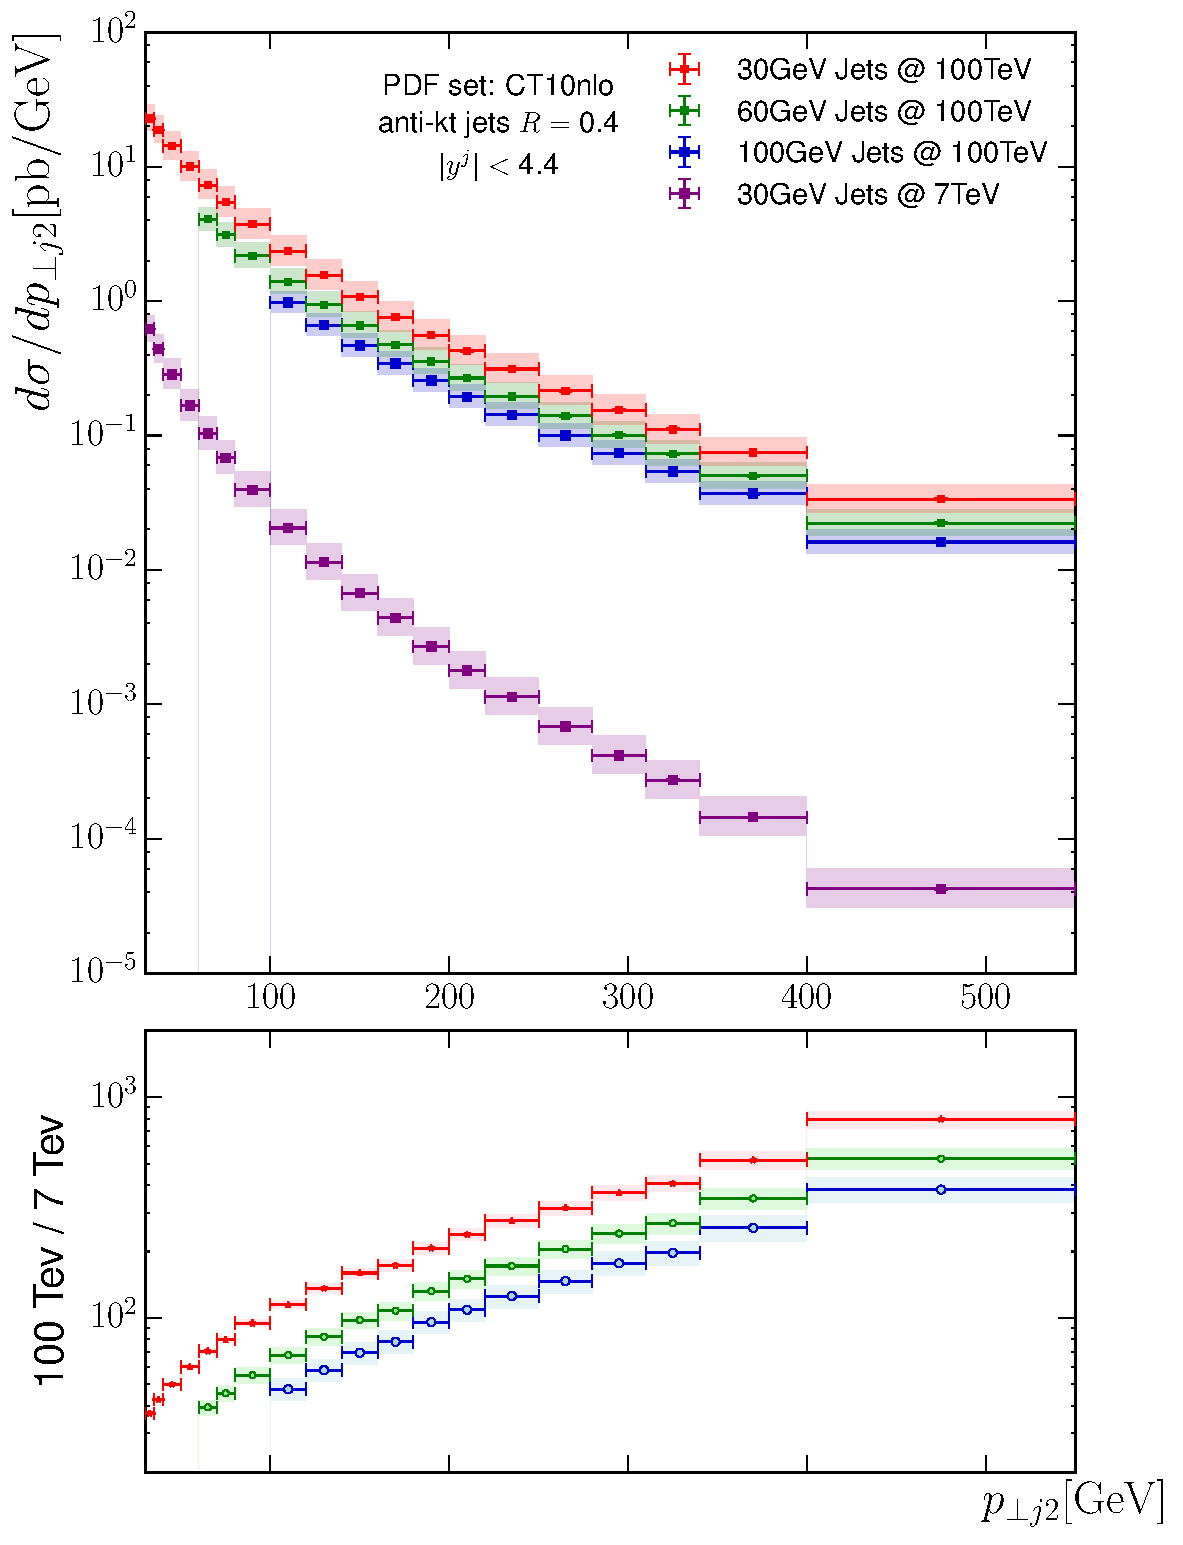
\includegraphics[width=\textwidth, height=1.3\textwidth]{ATLAS_Z_100TeV_5b}
			\caption{}
			\label{fig:100tev_5b}
		\end{subfigure}

		\begin{subfigure}[b]{0.48\textwidth}
			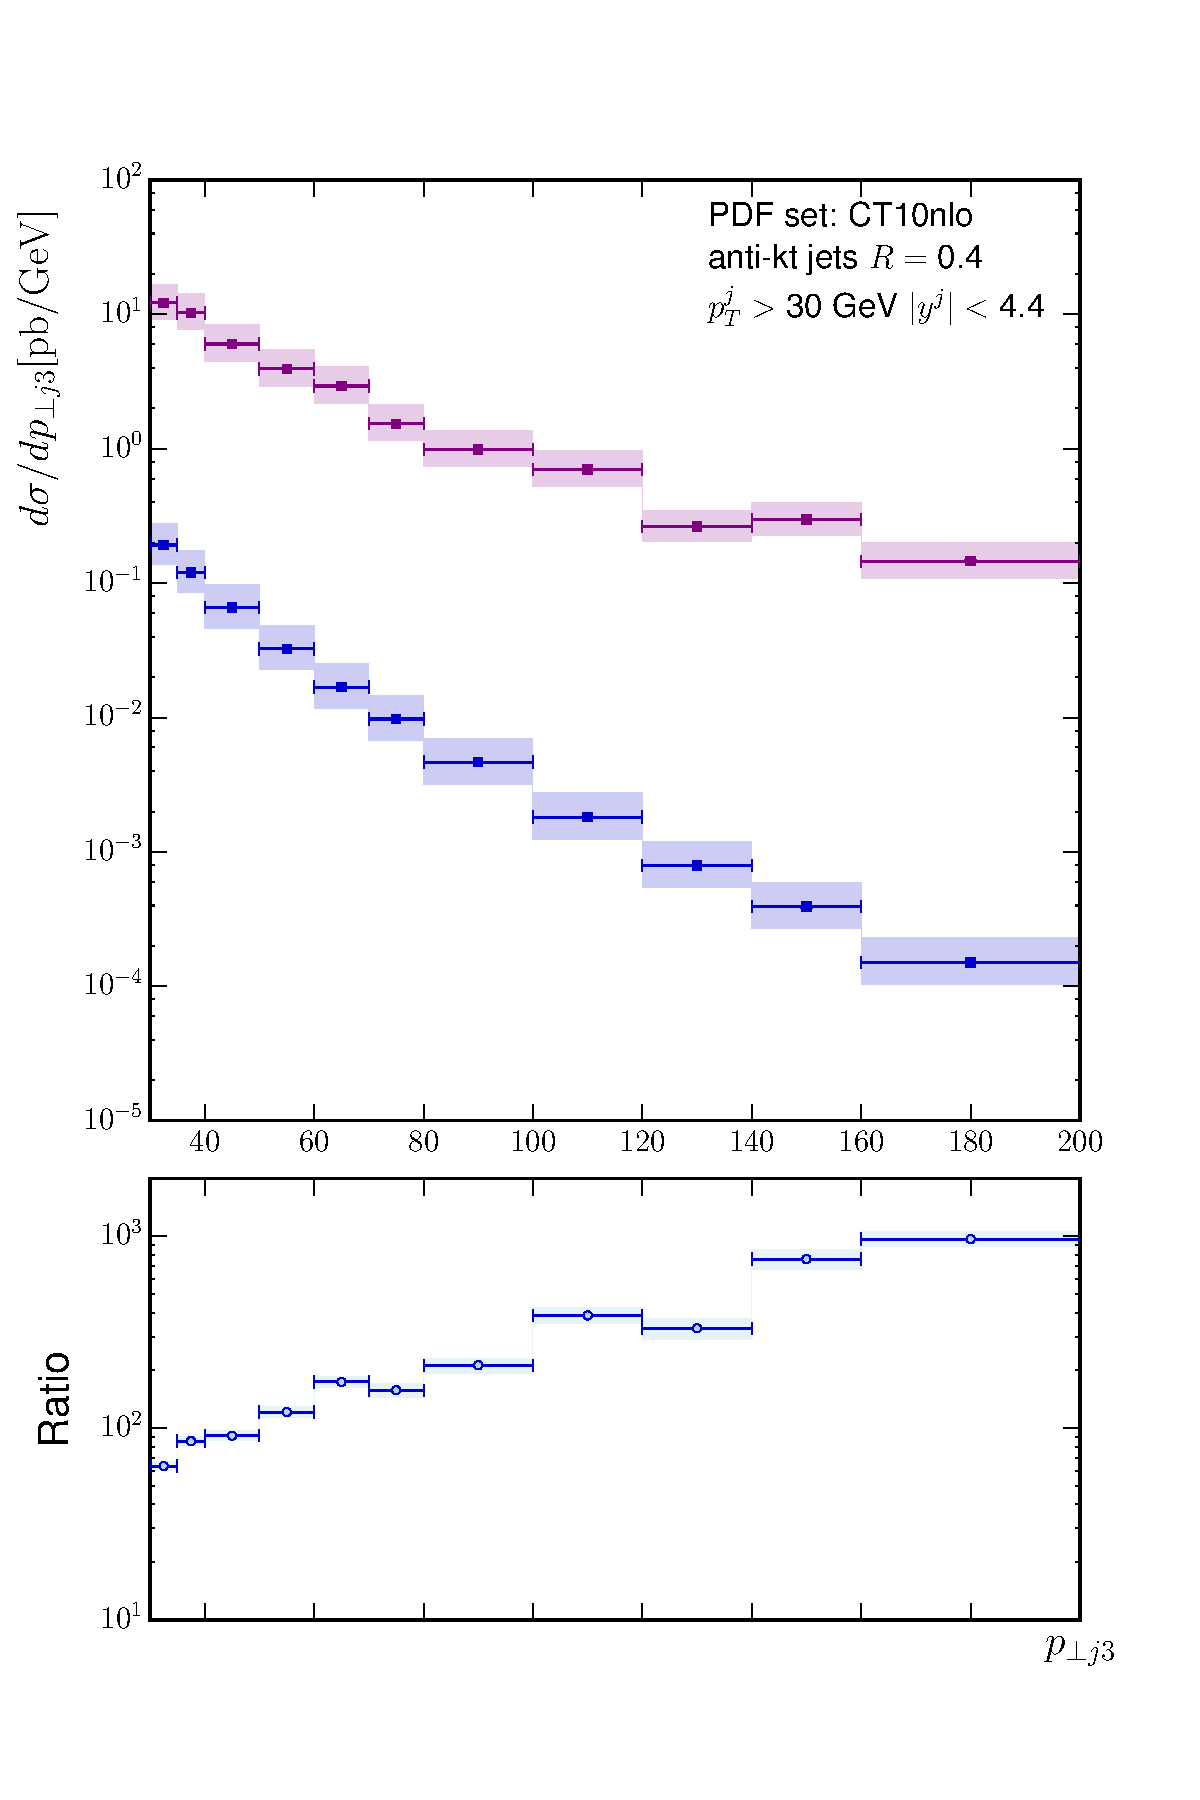
\includegraphics[width=\textwidth, height=1.3\textwidth]{ATLAS_Z_100TeV_6a}
			\caption{}
			\label{fig:100tev_6a}
		\end{subfigure}
		~
		\begin{subfigure}[b]{0.48\textwidth}
			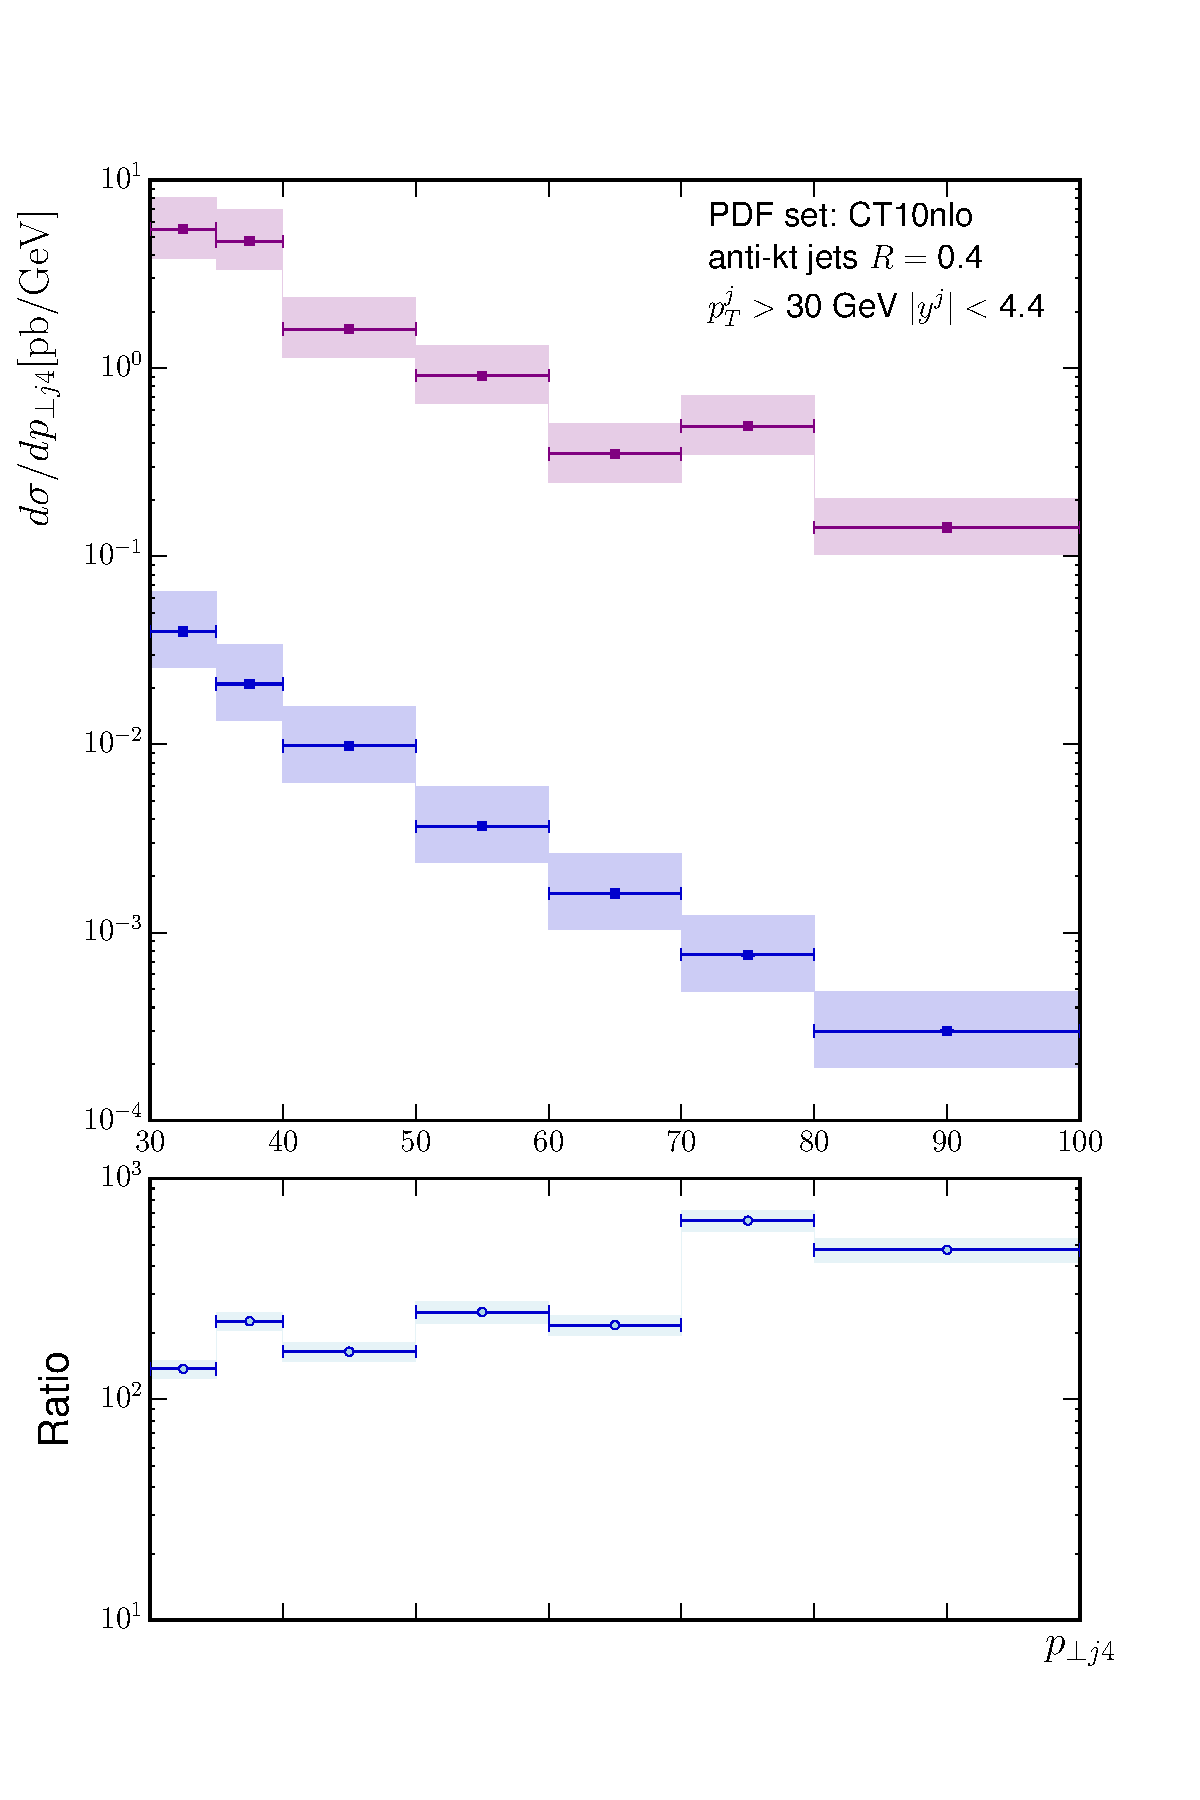
\includegraphics[width=\textwidth, height=1.3\textwidth]{ATLAS_Z_100TeV_6b}
			\caption{}
			\label{fig:100tev_6b}
		\end{subfigure}
		\caption{The differential cross-section for $\zg$ plus inclusive dijets as a function of the transverse momentum
		         of the first, second and third leading jets in $p_T$ shown in fig. \eqref{fig:100tev_5b}, \eqref{fig:100tev_6a}
		         and \eqref{fig:100tev_6b} respectively and for centre-of-mass energies of 7TeV (blue) and 100TeV (pink).}
	\end{figure}

	Fig. (\eqref{fig:100tev_5b}-\eqref{fig:100tev_6b}) notes:

	\begin{itemize}
		\item pT distributions,
		\item Heavy tails...soooo?
		\item More energy in initial state means we can get more jets further in to the outer regions of y-space,
		\item What effect would a shower have on these distributions?  Plenty of spare pT to radiate.
	\end{itemize}

	\begin{figure}[h]
		\centering
		\begin{subfigure}[b]{0.48\textwidth}
			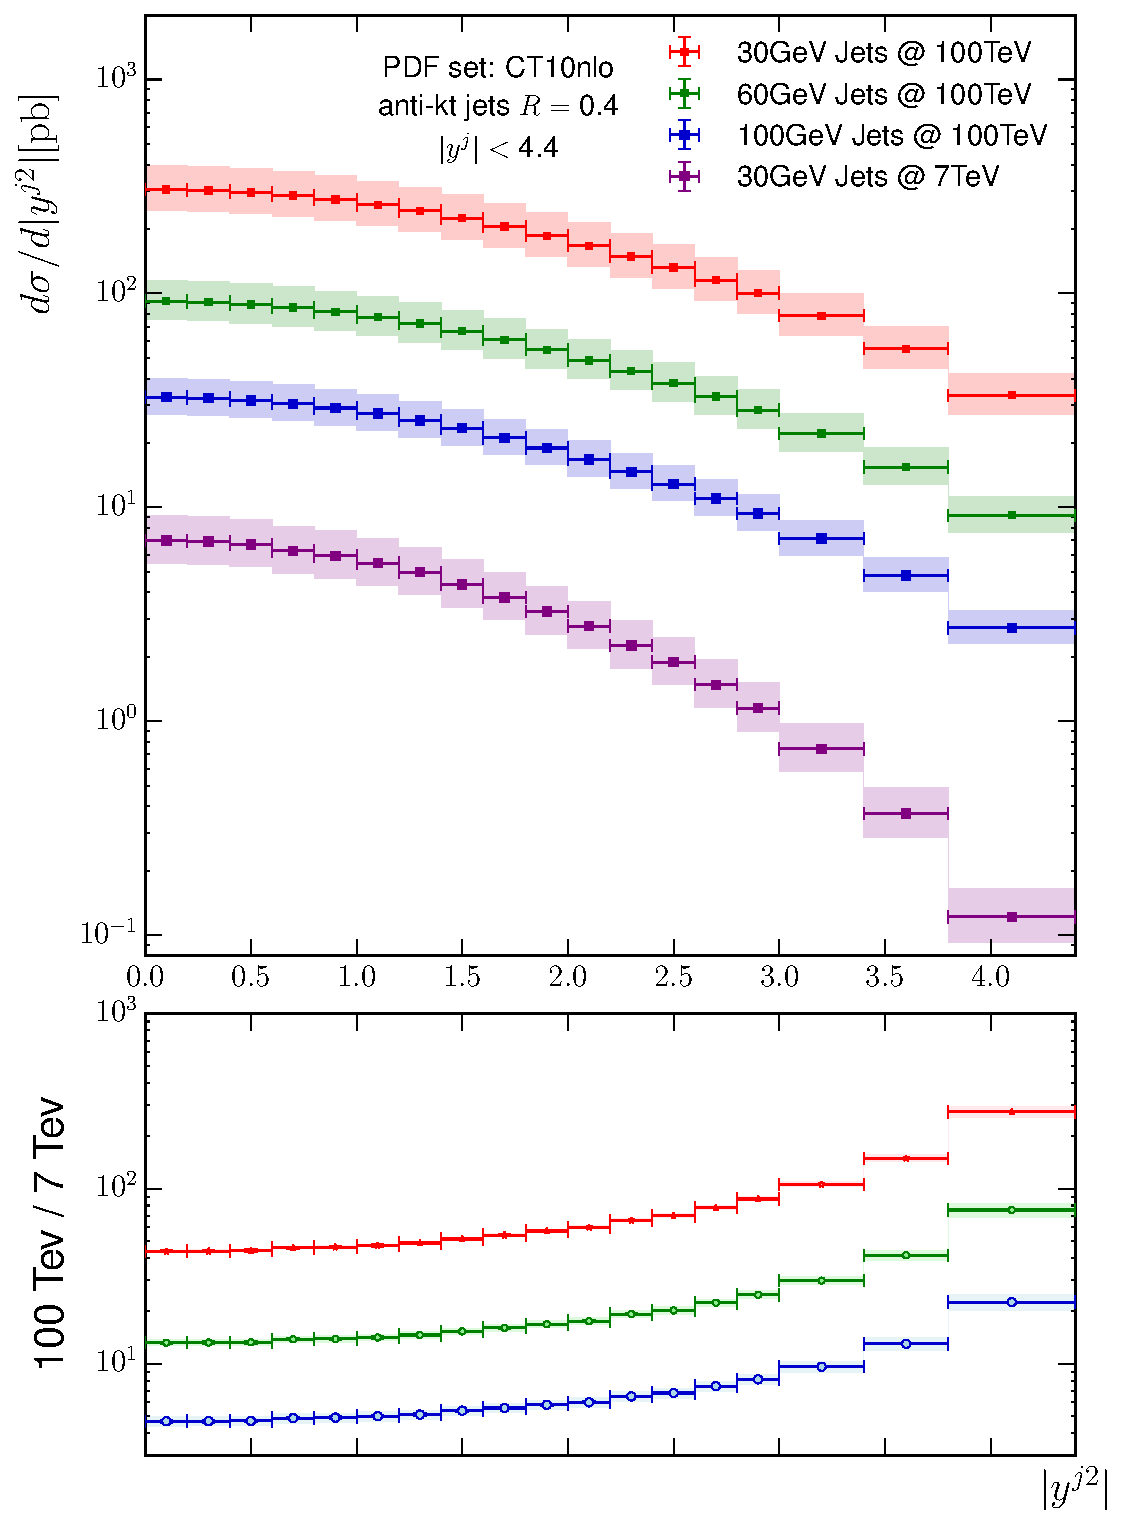
\includegraphics[width=\textwidth, height=1.3\textwidth]{ATLAS_Z_100TeV_9b}
			\caption{}
			\label{fig:100tev_9b}
		\end{subfigure}

		\begin{subfigure}[b]{0.48\textwidth}
			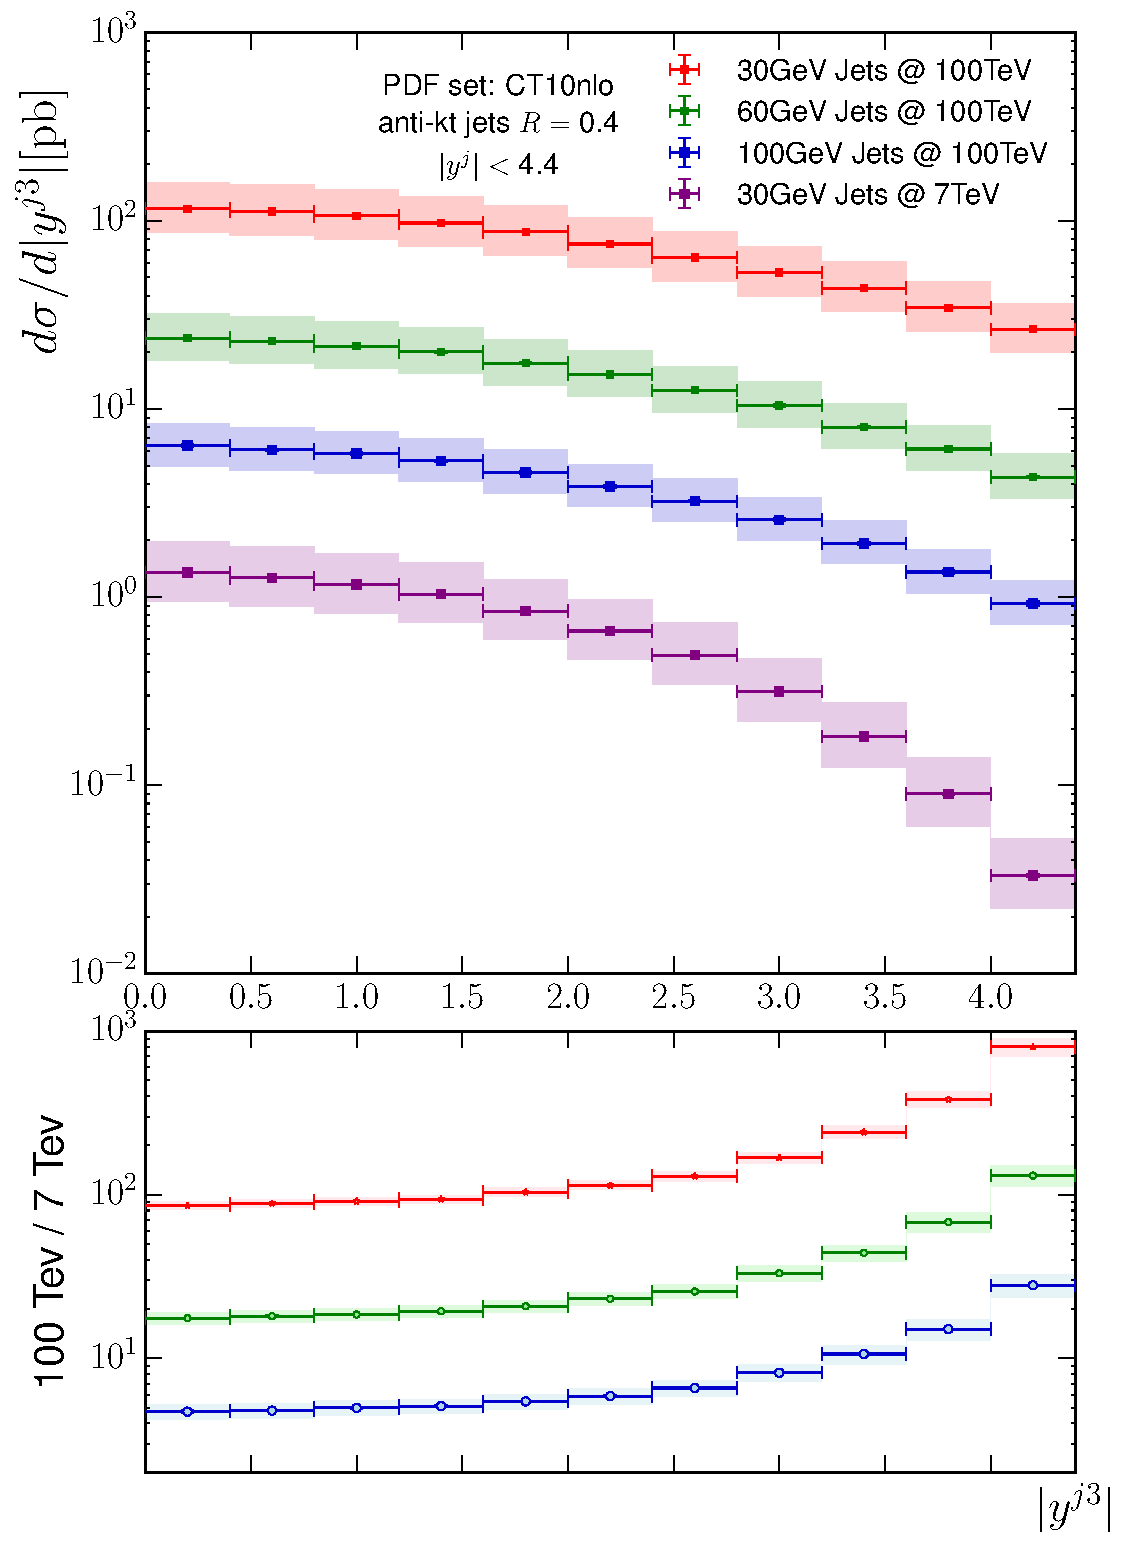
\includegraphics[width=\textwidth, height=1.3\textwidth]{ATLAS_Z_100TeV_10a}
			\caption{}
			\label{fig:100tev_10a}
		\end{subfigure}
		~
		\begin{subfigure}[b]{0.48\textwidth}
			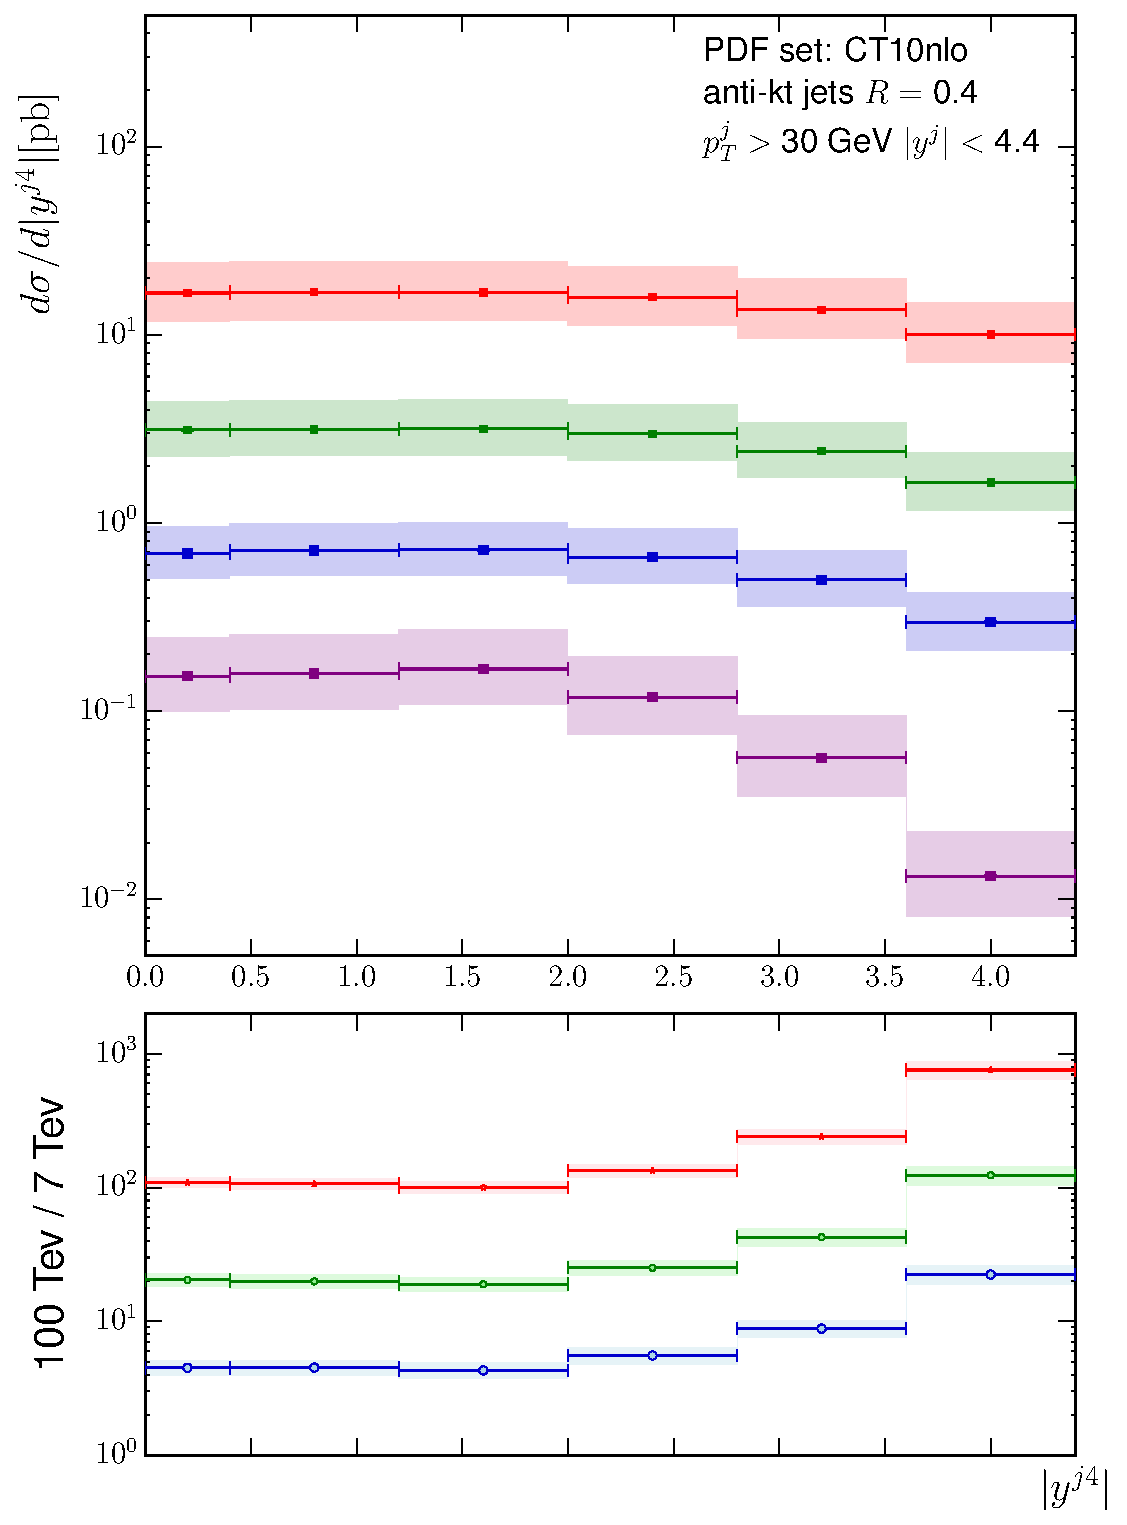
\includegraphics[width=\textwidth, height=1.3\textwidth]{ATLAS_Z_100TeV_10b}
			\caption{}
			\label{fig:100tev_10b}
		\end{subfigure}
		\caption{The differential cross-section for $\zg$ plus inclusive dijets as a function of the absolute value of the rapidity
		         of the first, second and third leading jets in rapidity shown in fig. \eqref{fig:100tev_9b}, \eqref{fig:100tev_10a}
		         and \eqref{fig:100tev_10b} respectively and for centre-of-mass energies of 7TeV (blue) and 100TeV (pink).}
	\end{figure}

	Fig. (\eqref{fig:100tev_9b}-\eqref{fig:100tev_10b}) notes:

	\begin{itemize}
		\item Not much more to say about these - mostly covered in dy plots,
	\end{itemize}

